\chapter{Theoretical Foundation}
\label{chap:theory}

\todo{More general introduction. Move the below to the SM section}

- Section underlines the theoretical underpinnings that manifest the Higgs boson as a special place in the universe

- Lots of SM parameters are related to Higgs (SM stands and falls with Higgs)

- The SM also has limitations -> precision measurements of Higgs required

- Many models of new physics expect to have access to new physics through interactions with Higgs ()

% From CARSTEN:
%This chapter outlines the Lagrange formulation of the Standard Model of Elementary Particle Physics (SM), a successful framework to study the fundamental laws governing the universe. Special attention is devoted to the Brout-Englert-Higgs (BEH) mechanism of electroweak symmetry breaking (EWSB). A more detailed introduction including all aspects of the model can be found in many textbooks [24–28].


\section{The Standard Model of Particle Physics}
\label{sec:sm}


% From Master's thesis:
The SM of particle physics is a collection of relativistic quantum field theories (QFT) that describe the interactions between all known fundamental particles.
Mathematically, it is a non-abelian gauge theory with the gauge group
\begin{equation}
  \label{eq:sm-gauge-group}
  \text{SU(3)}_C \times \text{SU(2)}_L \times \text{U(1)}_Y,
\end{equation}
the details of which are explained in this section.
% The mathematical formulation SU(3)$_C$ $\times$ SU(2)$_L$ $\times$ U(1)$_Y$ local gauge symmetry that gives rise to the interactions between all known fundamental particles.
%It evolved during the 60’s and 70’s due to a strong interplay between experimental observations and theoretical developments. 
\Cref{subsec:particle-content} provides a high-level overview of the particles and forces that are part of the SM. \Cref{subsec:formalism} briefly outlines the theoretical principles that build the basis for the mathematical description of the SM. \Cref{subsec:qed,subsec:qcd,subsec:ew-model,subsec:ewsymbreaking,subsec:fermion-masses,subsec:final-lagrangian} discuss the mathematical formulation of the SM, including a detailed description of the \emph{Higgs mechanism} of \emph{electroweak symmetry breaking} (EWSB).
The free parameters of the SM are discussed in \cref{subsec:free-pars-sm}, and \cref{subsec:limitations} concludes this section by summarizing the limitations and open questions of the SM.
% that motivate conducting more precise measurements such as the one presented in \cref{chap:hww} of this thesis.
The SM is covered in all its detail in the literature, e.g. \ccite{Peskin:1995ev,Halzen:1984mc,Thomson:2013zua}, which serve as the primary resources for the following descriptions.


% From previous theoretical foundation intro:
% - Section underlines the theoretical underpinnings that manifest the Higgs boson as a special place in the universe
% - Lots of SM parameters are related to Higgs (SM stands and falls with Higgs)
% - The SM also has limitations -> precision measurements of Higgs required
% - Many models of new physics expect to have access to new physics through interactions with Higgs ()


%On a phenomenological level, fundamental physics can be described in terms of elementary particles and forces. 
% - Introduction to QFT and gauge group
% - Lagrangian formalism
% - local gauge invariance: without local gauge invariance:

% From Pich The Standard Model
% Thus, once a given phase convention has been adopted at one reference point x0, the same convention must be taken at all space-time points. This looks very unnatural.

% - highly successful in describing QED
% WHAT HAPPENS IN THIS SECTiION:

% - First overview of particles and forces
% - Formalism
% - QED, QCD, electroweak model
% - Problem: no masses for bosons -> Higgs mechanism
% - Final Lagrangian and parameters to be measured experimentally of the SM
% - Limitations of the SM

\subsection{Particles and Forces}
\label{subsec:particle-content}

\begin{figure}
  \newImageResizeCustom{1}{figures/theory/particles-infographic/particles-infographic.pdf}
  \caption[Overview of particles in the SM.]{Overview of the particles in the SM. Their charge, color, mass, and spin are indicated. More details are given in the text. The graphic is adapted from \ccite{CBurgardParticlesInfographic} and the values taken from \ccite{PDG2020}.}  
  \label{fig:particles-infographic}
\end{figure}
\todo{Maybe put graphic on full page alone to make it bigger}
%In QFT all fundamental fields have an associated particle, that can be thought of as excitations (or vibrations) of the fields.
QFT describes nature in terms of fundamental fields and their interactions. Each field is associated with an elementary particle that can be thought of as a quantum excitation of the underlying field. 
This association makes it possible to describe fundamental physics using elementary particles.
%\footnote{To simplify terminology, the objects are mostly referred to as particles rather than fields in this chapter, but the relationship is important to be kept in mind.} 
% On a \TDnote{phenomenological}{other word?} level, fundamental physics can be described in terms of elementary particles and forces.
% All currently known particles and forces included in the SM are listed in \TDnote{REF}{REF}.
The particle content of the SM is summarized in \cref{fig:particles-infographic}. The particles can be grouped into two main types: 
\emph{fermions} with half-integer spin and \emph{bosons} with integer spin. The interaction between the fermions (sometimes called \emph{matter particles}) are interpreted as exchanges of \emph{gauge bosons} (also called \emph{force carriers}) that mediate the fundamental forces. 
% \emph{fermions} with half-integer spin (sometimes called \emph{matter particles}) and \emph{bosons} with integer spin (known as the \emph{mediators} or \emph{force carriers} of the fundamental forces).

The fermions can be grouped into three generations, each containing two leptons and two quarks. The different types of leptons and quarks are referred to as (quark or lepton) \emph{flavors}.
Quarks have an additional property called \emph{color}, which can take three possible values typically labelled as red, green, and blue\footnote{In fact, also linear combinations of the three colors are realized in nature, as discussed later in this chapter.}.
Additionally, each fermion has a corresponding antiparticle that has the same mass but ``opposite'' internal quantum numbers, that is, oppositely signed charge and anti-color if applicable.

%The interactions between the fermions can be described by exchanges of so-called \emph{gauge bosons}.
The SM includes three of the four known fundamental interactions: The \emph{electromagnetic interaction}, the \emph{strong interaction}, and the \emph{weak interaction}. The electromagnetic and the weak interactions are unified in the \emph{electroweak theory}. The fourth known fundamental interaction, \emph{gravitation}, is not part of the SM but can be fully neglected in present particle physics experiments due to its weak strength.
The gauge boson that mediates the electromagnetic interaction is the massless \emph{photon} that interacts with all charged fermions. Electromagnetic interactions are described by the theory of \emph{quantum electrodynamics} (QED). The strong interaction is transmitted via eight massless gluons, following the rules of \emph{quantum chromodynamics} (QCD). QCD acts on matter particles that carry color, that is, quarks and gluons themselves. 
Due to a property known as \emph{confinement} in QCD\footnote{Confinement arises because of the energy dependence of the strength of the QCD interactions, which is discussed in \cref{subsec:factorisation}.}, quarks cannot be found in isolation. They are confined within hadrons that consist, for example, of a quark and an anti-quark (known as \emph{mesons}) or three quarks (known as \emph{baryons}).
The weak interaction is mediated by three massive gauge bosons, \Wplus, \Wminus, and \Zboson, and acts on all fermions. Similar to gluons, the \Wpm and \Zboson bosons are able to interact with themselves.

The final particle of the SM is the electrically neutral \emph{Higgs boson}. It is the only spin-0 scalar particle and plays a special role in the SM in the mechanism of electroweak symmetry breaking through which the \Wpm and \Zboson bosons gain their masses. A dedicated overview of the physics involving the Higgs boson is provided in \cref{sec:higgs-phen}.


\subsection{Formalism and Principles}
\label{subsec:formalism}
% - Action: S = Int ( Lagrangian ) dt -> EOMs
% - Lagrangian = Int (Lagrange density ) d3x
% -> Lagrange density is commonly referred to as Lagrangian 
% - In QFT, we define EOMs for fields by specifying the Lagrange density (Lagrangian)

% ONE MORE SENTENCE:
% In physics, equations of motion are equations that describe the behavior of a physical system in terms of its motion as a function of time.[1] More specifically, the equations of motion describe the behavior of a physical system as a set of mathematical functions in terms of dynamic variables.

% Particles can be thought of as excitations (or vibrations) of corresponding fundamental fields. 
In order to describe the behaviour of a physical system, the equations of motions can be derived from the action,
\begin{equation}
  \label{eq:action}
  S = \int \Lagrangian d^3x dt,
\end{equation}
by following the action principle.\footnote{The derivation of the equations of motion can be found in any standard textbook on QFT, e.g. in \ccite{Peskin:1995ev}.}
The dynamics of a system are therefore fully specified by the Lagrange density, \Lagrangian. The Lagrange density, often simply denoted \emph{Lagrangian}, generally is a function of the fields $\psi$, and their derivatives $\partial \psi$, so $\Lagrangian \rightarrow \Lagrangian\left(\psi, \partial\psi\right)$. The fields are themselves generally dependent on the space-time coordinate, $\psi \rightarrow \psi(x)$.\footnote{For cleaner notation, these dependencies are not explicitly mentioned throughout this thesis.}

For a given field $\psi$, the principles of QFT demand to include all possible interaction terms in the Lagrangian that are related to the field\footnote{This follows what is sometimes referred to as the ``totalitarian principle'' of quantum mechanics, that satirically states: ``Everything not forbidden is compulsory'', meaning that everything allowed by the laws of physics must actually happen or exist.}.
The number and type of terms that can be included in the SM, however, is strongly constraint by requiring the theory to be invariant under symmetry transformations of the fields following the SM gauge group shown in \cref{eq:sm-gauge-group}.
The SM is governed by the principle of \emph{local gauge invariance}, which implies that the physical content of the theory stays the same when performing transformations of the particle fields,
\begin{equation}
  \psi \rightarrow e^{-iT} \psi,
\end{equation}
independently at every space-time point. Here, $T$ is the generator of a symmetry group which is generally dependent on the space-time coordinate, $T \rightarrow T(x)$. 
\todo{Maybe remove the transformation equation. A bit distracting/random here?}
% Gauge theories require the introduction of so-called gauge fields, that transform in a way so that the theory stays locally gauge invariant.
% Pich
% This is only possible if one adds an extra piece to the Lagrangian, transforming in such a way as to cancel the ∂μθ term in Eq. (6).
% In order to maintain the symmetry, the Lagrangian may need to be manipulated by introducing new fields.
Gauge theories require the addition of so-called gauge fields, which give rise to particle interactions that give rise to the fundamental forces of nature. 
Historically, the first local gauge theory that was established is QED. It follows a U(1) local gauge symmetry and entails the photon as the associated gauge field. 
The SM can be elegantly described by demanding local gauge invariance with the symmetry group as shown in \cref{eq:sm-gauge-group}, and explains the existence of all gauge bosons mentioned in the previous section. 
The fermions, in contrast, are added a priori to the theory and do not follow from fundamental principles.
%The following sections provide an overview of the Lagrangian of the SM, by going through the different symmetry groups. 
The following sections will outline the Lagrange formulation of the SM.
In all equations, natural units are used, that is, $c = \hbar = 1$, which leads to the mass, momentum, and energy of particles being expressed in units of electronvolt (\eV).
Moreover, the Einstein-summation convention is used, that is, terms with equal indices are considered to be summed. If not mentioned otherwise, greek-letter indices take integer values from 1 to 4, while latin-character indices take integer values from 1 to 3.

% - renormalization:
% We consider that the physics is understood up to a given cut-off/scale Lambda.

%The SM is governed by the principle of local gauge invariance and the associated symmetry group is SU(3)$_C$ $\times$ SU(2)$_L$ $\times$ U(1)$_Y$. 

% the next important lesson is that the existence of these symmetries places suck an incredibly strong constraint on what the theory actually is.

% Sean
% QED: demanding all the terms in your Lagrangian being gauge invariant is enforcing the conservation of electric charge gauge
% This is a reflection of Noethers theory. Symmetry conservation -> associated quantity of the U(1) symmetry is charge

% Sean Carrol:
% W and Z bosons are the physical excitations from vibrations in the SU(2) to gauge field
%the existence of these fields giving rise to interactions giving rise to forces of nature comes from the gauge symmetry.
% the next important lesson is that the existence of these symmetries places suck an incredibly strong constraint on what the theory actually is.

% From Master thesis
% An essential part of the mathematical formulation of the SM is based on the postulation of local gauge invariance. It implies, that the physical content of the theory should stay the same when performing certain redefinitions of the particle fields independently at every space-time point. The SM follows a SU(3)×SU(2)L×U(1)Y symmetry group, where SU(3) is the gauge group of QCD and SU(2)L×U(1)Y the corresponding symmetry for the electroweak model (the meaning of the subindizes L and Y will be explained in the following sections). Historically, QED was the first well established gauge theory, following a U(1) symmetry. To demonstrate the principles of a gauge theory, which are the key concepts of the mathematical framework of the SM, the QED Lagrangian will be derived in the following. Subsequently the same principles are applied to describe the main aspects of the more complex theories of QCD and the electroweak model. A description of the mechanism to incorporate masses for the W± and Z bosons via breaking the electroweak symmetry is given thereafter. The following sections follow to a large extend the more detailed descriptions given in Refs. [19–21].


\subsection{Quantum electrodynamics}
\label{subsec:qed}
%The above derivations are shortly recapped: Starting from the Lagrangian of a freely moving relativistic fermion one can impose the requirement of local U(1) gauge invariance. This demands to add a new field $A_\mu$ toghether with an interaction term, which is incorporated in the Lagrangian by introducing a covariant derivative $D_\mu$. Additionally, the kinetic term in \cref{eq:kinetictermqed} needs to be added for the new field, which leads to the final Lagrangian for QED, shown in \cref{eq:Lagrangianqed}.
\todo{Explain w(x) in the equation and does it need to be bold x?}
QED can be regarded as a reflection of an underlying $U(1)$ local gauge symmetry of the complex-valued fermion fields, $\psi_f$, known as \emph{Dirac spinors}.
The Lagrangian that is invariant under $\psi_f \rightarrow e^{i \omega(x)} \psi_f$ transformations can be written as
\begin{equation}
  \mathcal{L}_{\text{QED}} = \sum_f \bar{\psi}_f(i\gamma^\mu D_\mu - m_f)\psi_f - \frac{1}{4}F_{\mu\nu}F^{\mu\nu},
  \label{eq:Lagrangianqed}
\end{equation}
where the sum goes over all electrically charged fermions with masses $m_f$, and $\gamma^\mu$ refers to the four $4 \times 4$ gamma matrices.
Here, $D_\mu$ is the \emph{covariant derivative} defined as
\begin{equation}
  D_\mu = \partial_\mu + ieA_\mu,
\end{equation}
which includes the gauge field $A_\mu$ that is associated with the photon. The requirement of local gauge symmetry prohibits terms quadratic in $A_\mu$, resulting in the prediction of the photon being massless.\footnote{Terms in the Lagrangian that are quadratic in a certain field give rise to particle masses.}
The so-called \emph{field tensor} is defined as
\begin{equation}
  F_{\mu\nu} = \partial_\mu A_\nu - \partial_\nu A_\mu,
\end{equation}
where $\partial_\mu$ are the partial derivatives. This tensor provides an elegant mathematical object representing the electromagnetic field and can also be used, for example, to describe Maxwell's equations of classical electrodynamics.

The symmetry group associated to QED is denoted U(1)$_{\text{QED}}$ and the conserved quantity is the electric charge.\footnote{This is a reflection of Noether's theorem, which states that each symmetry is related to a conserved quantity.}
It should be noted that U(1)$_{\text{QED}}$ is not part of the original symmetry group of the SM. As explained below, U(1)$_{\text{QED}}$ arises from a SU(2)$_L$ $\times$ U(1)$_Y$ symmetry that is spontaneously broken.


\subsection{Quantum chromodynamics}
\label{subsec:qcd}
QCD is a non-abelian gauge theory associated to a SU(3)$_C$ symmetry. The subindex $C$ refers to the color which is the conserved quantity under SU(3)$_C$ transformations.
The locally gauge invariant QCD Lagrangian reads
\begin{equation}
  %  \mathcal{L}_{\text{QCD}} = -\frac{1}{4}G_{\mu\nu}^aG^{a\,\mu\nu} + \bar{q}^i\left( i\gamma^\mu D_\mu-m \right)^j_i q_j,
  \mathcal{L}_{\text{QCD}} = \sum_f \bar{\psi}_f(i\gamma^\mu D_\mu - m_f)\psi_f - \frac{1}{4}G_{\mu\nu}^aG^{\mu\nu}_{a},  \label{eq:lqcd}
\end{equation}
where the sum runs over all quark fields, $\psi_f$, that take the form of spinor triplets. 
\todo{Sum over A in lambdaA GmuA in the equation?}
The covariant derivate is given by
\begin{equation}
    D_\mu = \partial_\mu + i g_s \frac{\lambda^a}{2} G_\mu^a,
\end{equation}
which includes eight gluon fields $G_\mu^a$ (with $a = 1, \ldots, 8$), the strong coupling constant $g_s$, and the Gell-Mann matrices $\lambda^a$ that are the generators of the SU(3)$_C$ group.
The field tensors $G_{\mu\nu}^a$ are defined as
\begin{equation}
  \label{eq:qcd-tensor}
  G_{\mu\nu}^a = \partial_\mu G_\nu^a - \partial_\nu G_\mu^a - g_s f^{abc}G_\mu^b G_\nu^c,
\end{equation}
where $f^{abc}$ are the structure constants of SU(3)$_C$. 
The last term in \cref{eq:qcd-tensor} arises from the non-commuting elements of the SU(3)$_C$ group and gives rise to triple and quartic gluon self-interactions. 
% Triple and quartic self-interactions are part of QCD because gluons themselves carry a combination of a color and anti-color. 
% Invariant under ... transformation, where ... are the group generators
Similar to photons, the gluons are massless because no terms quadratic in the gluon fields are allowed when requiring local gauge invariance. 
%which is similar to the requirement of a massless photon in QED. 



\subsection{The electroweak model}
\label{subsec:ew-model}
  \begin{table}
    \caption[Overview of the fermion content in the electroweak model.]{Overview of the fermion content in the electroweak model with the quantum numbers of the weak isospin $T^3$, hypercharge $Y$ and electric charge $Q$. They are grouped into left-handed doublets and right-handed singlets denoted with the subindex $L$ and $R$ respectively. The down-type quarks $d', s', b'$ are the eigenstates of the electroweak interaction and given by linear combinations of the mass eigenstates $d, s, b$. This mixing is described by the CKM matrix, see text. Since right-handed neutrinos are not undergoing any interaction they do not play a role in the Standard Model and are not listed here.}
    \label{tab:ewfermioncontent}
    \centering
      \begin{tabular}{c |@{}| c c c | c c c}
        \toprule
                                 & \multicolumn{3}{c}{Generation}          & \multicolumn{3}{|c}{Quantum number}                                                                                                            \\
                                 & 1$^{\text{st}}$                         & 2$^{\text{nd}}$                             & 3$^{\text{rd}}$                               & $T^3$          & $Y$            & $Q$            \\
        \midrule
        \multirow{3}{*}{Leptons} & \multirow{2}{*}{$\myvec{\nu_e                                                                                                                                                            \\ e}_L$} & \multirow{2}{*}{$\myvec{\nu_\mu \\ \mu}_L$} & \multirow{2}{*}{$\myvec{\nu_\tau \\ \tau}_L$} & $\frac{1}{2}$  & -1             & 0 \\
                                 &                                         &                                             &                                               & $-\frac{1}{2}$ & -1             & -1             \\
                                 & $e_R$                                   & $\mu_R$                                     & $\tau_R$                                      & 0              & -2             & -1             \\
        \midrule
        \multirow{3}{*}{Quarks}  & \multirow{2}{*}{$\myvec{u                                                                                                                                                                \\ d'}_L$}    & \multirow{2}{*}{$\myvec{c \\ s'}_L$}        & \multirow{2}{*}{$\myvec{t \\ b'}_L$}          & $\frac{1}{2}$  & $\frac{1}{3}$  & $\frac{2}{3}$ \\
                                 &                                         &                                             &                                               & $-\frac{1}{2}$ & $\frac{1}{3}$  & $-\frac{1}{3}$ \\
                                 & $u_R$                                   & $ c_R$                                      & $t_R$                                         & 0              & $\frac{4}{3}$  & $\frac{2}{3}$  \\
                                 & $d_R$                                   & $ s_R$                                      & $b_R$                                         & 0              & $-\frac{2}{3}$ & -$\frac{1}{3}$ \\
        \bottomrule
      \end{tabular}
  \end{table}



% - the chirality can be determined with... right-chiral fermions are singlets under SU(2)L transformations
% - This also means that no right-chiral neutrinos exist in the SM as they don't interact with any of the forces

% "Also called: The Glashow􏰁Weinb erg􏰁Salam Theory of Weak Interactions"
The weak and electromagnetic forces are unified in the electroweak model~\cite{GLASHOW1961579,SALAM1964168,PhysRevLett.19.1264} by imposing local gauge invariance under transformations of the symmetry group
\begin{equation}
  \label{eq:ew-sym-group}
  \text{SU(2)}_L \times \text{U(1)}_Y.
\end{equation}
The electroweak gauge group is based on two major empirical findings:
The first is, that only \emph{left-chiral}\footnote{
  The \emph{chirality} of a fermion can be determined with the projection operators $P_L$ and $P_R$ like
  \begin{equation*}
    \psi       = P_L \psi + P_R \psi = \frac{1}{2} \left( 1 - \gamma^5 \right) \psi + \frac{1}{2} \left( 1 + \gamma^5 \right) \psi = \psi_R + \psi_L,                                \\
  \end{equation*}
  where $\gamma^5 = i\gamma^0\gamma^1\gamma^2\gamma^3$. The chirality becomes identical to the helicity for massless particles.
} (also denoted \emph{left-handed}) fermions interact via the weak interaction, indicated with an $L$ in \cref{eq:ew-sym-group}. An overview of the fermion content is shown in \cref{tab:ewfermioncontent}, that groups the fermions into left-handed doublets, $\psi_L$, and right-handed singlets, $\psi_R$, under SU(2)$_L$ transformations. 
The second finding is that the quarks participating in the electroweak interaction, labelled as $u', d', c'$, are a mixture of the quark mass eigenstates. Their relation is specified by the \emph{Cabibbo–Kobayashi–Maskawa (CKM) matrix} \cite{doi:10.1143/PTP.49.652}, $\pmb{V}$, as
% From Peskin
% The off diagonal terms in Vij allow weak􏲩interaction transitions b e􏲩 tween quark generations.
\begin{equation}
  \begin{pmatrix}
   d' \\
   s' \\
   b'
 \end{pmatrix}
 = 
 \pmb{V} 
 \begin{pmatrix}
   d \\
   u \\
   b
 \end{pmatrix}.
\end{equation}
The CKM matrix is unitary and fully specified with 4 parameters and encodes the strength of the flavor-changing electroweak interactions.
\todo{Maybe add one more sentence describing the rotation that is necessary? see P.Sommer thesis}

\noindent The fermion fields then transform as
\begin{align}
  \psi_L & \rightarrow e^{iY\omega} e^{iT^a\omega^a} \psi_L, \qquad (a = 1, 2, 3) \\
  \psi_R & \rightarrow e^{iY\omega} \psi_R,
\end{align}
under SU(2)$_L$ $\times$ U(1)$_Y$ transformations, where $T^a=\frac{\sigma^a}{2}$ are the Pauli matrices and generators of the SU(2)$_L$ group.
The associated conserved quantity is the \emph{weak isospin} $T$, of which the third component is conserved in weak interactions and given by $T^{(3)} = \pm \frac{1}{2}$ for SU(2)$_L$ doublets and $T^{(3)} = 0$ for SU(2)$_L$ singlets.
The U(1)$_Y$ symmetry is associated to the \emph{hypercharge} $Y$, and cannot be directly associated to the QED gauge group.
The relation to the electromagnetic interaction and the physical electric charge $Q$ is
\begin{equation}
  Q = T^{(3)} + \frac{Y}{2}.
\end{equation}

\noindent The local gauge invariant electroweak Lagrangian can be written as
\begin{equation}
  \mathcal{L}_{\text{EWK}} = \sum_f i\bar{\psi}_{f}\gamma^\mu D_\mu \psi_{f} - \frac{1}{4}W_{\mu\nu}^aW^{\mu\nu}_{a} - \frac{1}{4} B_{\mu\nu}B^{\mu\nu}, 
  \label{eq:lagrangianewk}
\end{equation}
where the sum runs over all fermions $f$, including their left-handed and right-handed counterparts.
%, whose occurrence as left-handed and right-handed particles is explicitly mentioned.
The covariant derivative is defined as
\begin{equation}
  D_\mu = \partial_\mu + igT^aW_\mu^a + ig'\frac{Y}{2}B_\mu 
  \label{eq:covdevewk}
\end{equation}
and includes four gauge fields. The fields $W^a_\mu$ (with a = 1, 2, 3) are the gauge fields of SU(2)$_L$ with associated coupling $g$, and $B_\mu$ is the gauge field of U(1)$_Y$ with coupling $g'$.
The field tensors in \cref{eq:lagrangianewk} are given by
\begin{align}
  W_{\mu\nu}^a & = \partial_\mu W_\nu^a - \partial_\nu W_\mu^a - g \epsilon^{abc} W^b_\mu W^c_\nu, \label{eq:Wtensor} \\
  B_{\mu\nu}   & = \partial_\mu B_\nu - \partial_\nu B_\mu,
\end{align}
where $\epsilon^{abc}$ are the structure constants of SU(2)$_L$. The third term on the right-hand side of \cref{eq:Wtensor} arises because of the non-abelian nature of SU(2)$_L$ and gives rise to triple and quartic self-interactions of the gauge fields $W_{\mu}^a$.
The tensor $B_{\mu\nu}$ has the same structure as the electromagnetic field strength tensor obtained in QED.
\todo{Give details on structure constants? for QCD AND Electroweak model}

\noindent The Lagrangian of \cref{eq:lagrangianewk} describes 4 massless bosons. No terms quadratic in the vector fields are allowed due to the requirement of local gauge invariance. 
Another mechanism is required to explain the existence of the masses of the gauge fields \Wpm and \Zboson.
% and $\gamma$. 


% From experiments one expects two charged bosons $W^\pm$ and two neutral bosons, the $Z$ and the photon.

\subsection{Spontaneous symmetry breaking and the Higgs mechanism}
\label{subsec:ewsymbreaking}
%- Local gauge invariance does not allow adding mass terms
%- The SU(2)$_L$ $\times$ U(1)$_Y$ symmetry is spontaneously broken into U(1)$_\text{QED}$
%- This mechanism is spontaneous symmetry breaking
%- Simply put, the Lagrangian itself maintains the symmetry, but the state of lowest energy is not invariant and breaks the summetry.
% - Could add mass terms disregarding local gauge invariance but this would render theory unrenormalizable
\begin{figure}
  \newImageResizeCustom{0.75}{figures/theory/higgs-potential/higgs-potential.pdf}
  \caption[Two dimensional Higgs potential $V(\phi)$ with $\lambda > 0$ and $\mu^2 < 0$.]{Two dimensional Higgs potential $V(\phi)$ as in \cref{eq:higgspotential} with $\lambda > 0$ and $\mu^2 < 0$. The minimum occurs for different points on the sketched circle in the $(\phi_1, \phi_2)$ plane and has the value given in \cref{eq:higgsminima}.
  }
  \label{fig:higgspotential}
\end{figure}

%naturally appear in the Higgs mechanism explained below.
%An additional mechanism is needed in the SM to explain the finite masses of the weak gauge bosons. 

A principle known as \emph{spontaneous symmetry breaking}, that was first explored in the field of condensed-matter physics, can be applied to elementary particle physics to generate mass terms for the weak gauge bosons without violating local gauge invariance.
This was first formulated by three independent research teams in 1964: Brout and Englert~\cite{PhysRevLett.13.321}, Higgs~\cite{PhysRevLett.13.508,HIGGS1964132}, and Guralnik, Hagan, and Kibble \cite{PhysRevLett.13.585}.\footnote{Their work was inspired by previous advancements in the theory of superconductivity~\cite{PhysRev.108.1175} and specifically P. W. Anderson, who proposed the mechanism of spontaneous symmetry breaking for generating mass terms in a non-relativistic scenario already in 1963~\cite{PhysRev.130.439}.}
Today the mechanism is most often called \emph{Higgs mechanism} or \emph{electroweak symmetry breaking} (ESWB).
The basic principle is to allow the state of lowest energy to violate local gauge invariance while maintaining the gauge symmetry of the Lagrangian itself.

% From Peskin and Schroeder
% - In the theory of sup erconductiv􏰁 ity􏰔 for example􏰔 the Ab elian gauge invariance of electromagnetism is broken by pairs of electrons that condense in the ground state of a metal􏰎
%The mechanism is known as the \emph{Brout-Englert-Higgs mechanism} (or simply \emph{Higgs mechanism}) or also \emph{electroweak symmetry breaking} (ESWB).
%The underlying concept is that the Lagrangian itself maintains the symmetry, but the state of lowest energy is not invariant and breaks the gauge symmetry.
% was published almost simultaneously by three independent groups in 1964: by Robert Brout and François Englert;[3] by Peter Higgs;[4] and by Gerald Guralnik, C. R. Hagen, and Tom Kibble.[5][6][7]

The Higgs mechanism assumes a complex scalar field of the SU(2)$_L$ group,
\begin{equation}
  \phi = \frac{1}{\sqrt{2}} \myvec { \phi_1 + i \phi_3 \\ \phi_2 + i \phi_4},
\end{equation}
and introduces a potential of the form
\begin{equation}
  V(\phi) = \mu^2\phi^\dagger\phi + \lambda \left(\phi^\dagger\phi \right)^2.
  \label{eq:higgspotential}
\end{equation}
The Lagrangian 
\begin{equation}
  \mathcal{L}_{\text{Higgs}} = |D_\mu\phi|^2 - V(\phi), % - \frac{1}{4} W_{\mu\nu}^a W^{a\, \mu\nu} - \frac{1}{4} B_{\mu\nu} B^{\mu\nu},
  \label{eq:lagrangianhiggs}
\end{equation}
where $D_\mu$ is defined as shown in \cref{eq:covdevewk}, is invariant under local SU(2)$_L$ $\times$ U(1)$_Y$ transformations.
The parameters of the potential $V(\phi)$ are specifically chosen to satisfy $\mu^2 < 0$ and $\lambda > 0$.
This choice provides the \emph{Higgs potential} with a characteristic shape, depicted in \cref{fig:higgspotential}, and gives rise to a set of degenerate ground state configurations satisfying
\begin{equation}
  |\phi| = \sqrt{ \frac{\mu^2}{2\lambda} } \equiv \frac{ v }{\sqrt{2}},
  \label{eq:higgsminima}
\end{equation}
where $v$ is the non-zero \emph{vacuum expectation value} of the Higgs field.
%% We find that the Lagrangian for such a field
%% \begin{equation}
%% \end{equation}
%% is invariant under global SU(2) phase transformations
%It is invariant under gauge transformations but not the ground state, which can be found at
%The minimum of the potential can be found on the circle of minima where
%Once a ground state is chosen, the SU(2)$_L$ $\times$ U(1)$_Y$ symmetry becomes spontaneously broken.
% The symmetry is therefore spontaneously broken when a ground state is chosen. 
%The arbitrary choice of a ground state is said to spontaneously break the symmetry. 
Without loss of generality the ground state can be chosen to be
\begin{equation}
  \phi_0 = \frac{1}{\sqrt{2}} \myvec{0 \\ v},
  \label{eq:groundstate}
\end{equation}
that is, $\phi_1 = \phi_2 = \phi_4 = 0$ and $\phi_3 = \frac{v}{\sqrt{2}}$, which spontaneously breaks the SU(2)$_L$ $\times$ U(1)$_Y$ symmetry.
Expanding the field $\phi$ around the minimum to first order in the fields yields
\begin{equation}
  \phi(x) = e^{i\frac{\phi(x)}{v}}\frac{1}{\sqrt{2}} \myvec{ 0 \\ v + h(x) },
    \label{eq:higgsexp}
\end{equation}
where the extra term $e^{i\frac{\phi(x)}{v}}$ describes the fluctuations of the fields $\phi_1, \phi_2, \phi_4$ around the vacuum $\phi_0$.
These fields are known as the \emph{Goldstone bosons} and have no direct physical implications. They can be eliminated from the Lagrangian by choosing an appropriate gauge, the \emph{unitary gauge}, so that 
\begin{equation}
  \phi(x) = \frac{1}{\sqrt{2}} \myvec{ 0 \\ v + h(x) }.
  \label{eq:expanded-groundstate}
\end{equation}
There remains only one real physical field, $h(x)$, which is called the \emph{Higgs field} and is associated with a neutral scalar boson, the \emph{Higgs boson}, labelled $H$.
The mass of the Higgs boson follows by inserting \cref{eq:expanded-groundstate} into \cref{eq:higgs-potential},
\begin{equation}
  m_H = \sqrt{2} \mu = \sqrt{2 \lambda} v.
\end{equation}
Inserting \cref{eq:higgsexp} into \cref{eq:lagrangianhiggs} and using the linear combinations,
\begin{align}
  W_\mu^\pm &= \frac{1}{\sqrt{2}} \left( W_\mu^1 \mp iW_\mu^2 \right),  \\
  Z_\mu &= \cos\theta_\text{w} W_\mu^3 - \sin\theta_\text{w} B_\mu, \\
  A_\mu &= \cos\theta_\text{w} B_\mu - \sin\theta_\text{w} W_\mu^3,
\end{align}
where $\theta_\text{w}$ is the \emph{weak mixing angle} defined as $\sin\theta_\text{w}^2 = \frac{g'^2}{g^2+g'^2}$, leads to the following terms in the Lagrangian
\begin{equation}
  \mathcal{L}_m = \frac{1}{4} \left( v + H \right)^2  \left(g^2 W_\mu^+W^{-\,\mu} + \frac{g^2}{2\cos\theta_\text{w}^2} Z_\mu Z^\mu \right).
  \label{eq:lagrangianmasses}
\end{equation}
One can identify terms quadratic in the physical fields $\Wpm$ and $Z$, generated by the non-vanishing expectation value $v$, giving rise to the masses
\begin{align}
  m_W &= \frac{vg}{2}, \\
  m_Z &= \frac{m_W}{\cos \theta_\text{w}},
  \label{eq:boson-masses}
\end{align}
of the weak gauge bosons.
The mass of the $W$ boson can be related to the Fermi constant, $G_F$, via $m_W = \frac{g}{4 * \sqrt{2}G_F}$. 
No field quadratic in $A_\mu$ appears, which reflects the fact that the photon is massless.

% DIFFERENT Formulation: It is worth while to decompose the Lagrangian into its different pieces:
The Lagrangian in \cref{eq:lagrangianmasses} can be re-written after substituting the masses of the gauge bosons,
\begin{equation}
  \mathcal{L}_{\text{H,boson-coupling}} = m_W^2 W_\mu^+W^{-\,\mu} \left( \frac{2H}{v} + \frac{H^2}{v^2} \right) + \frac{1}{2} m_Z^2 Z_\mu Z^\mu \left( \frac{2H}{v} + \frac{H^2}{v^2} \right),
  \label{eq:higgsbosoncoupling}
\end{equation}
which shows that the interaction between the Higgs boson and the massive gauge bosons is proportional to the square of the mass of the coupled bosons and involves triplet ($V^\dagger VH$) and quartic ($V^\dagger VHH$) couplings.

%and choosing a specific gauge (the unitary gauge) the field $\phi$ can be written as
% As shown below, introducing a complex SU(2)$_L$ doublet does not only give rise to the $\Wpm$ and $Z$ boson masses, but can also be used to construct mass terms for fermions. Hence, the Higgs field couples to all massive elementary particles.
% A more detailed descriptions on experimental Higgs boson physics and an overview of the current state of knowledge is given in \cref{sec:higgsphysics}.
% The parameters of the Higgs potential $\mu^2 = \lambda v^2$ can be fixed for one combination by measuring parameters of the electroweak theory, but the physical Higgs mass cannot be predicted. 
% Moreover, the last two terms in \cref{eq:higgsselfcoupling} predict that the Higgs field couples to itself with cubic and quartic interactions.
% The couplings of the Higgs boson to the weak gauge bosons are already expressed in \cref{eq:lagrangianmasses}.

%While the Higgs boson was discovered experimentally in 2012 \cite{Aad:2012tfa,Chatrchyan:2012xdj}, and is by now seen in several different production and decay modes, the Higgs boson self-couplings are still searched for.


% In summary, adding a complex scalar Higgs field to the electroweak model, together with a potential that exhibits a non-zero vacuum expectation value, provides the ingredients to obtain mass terms for the weak gauge bosons $W^\pm$ and $Z$ when choosing a ground state of the Higgs field which spontaneously breaks the symmetry.
% The three Goldstone bosons that arise can be eliminated from the Lagrangian by using its underlying local gauge symmetry. 
% This results in three bosons acquiring a mass and the appearance of one remaining scalar field $H$. 
% The photon remains massless, because the U(1)$_{\text{QED}}$ symmetry is unbroken. 


\subsection{Fermion masses}
\label{subsec:fermion-masses}
\todo{Maybe add in the beginning that simple inclusion of fermion mass terms is forbidden in electroweak model. As commented out at the end of the EW section.}

The previous section explained how the Higgs mechanism naturally gives rise to mass terms for the $\Wpm$ and $Z$ bosons. The finite fermion masses, however, do not directly follow and the simple inclusion of fermion mass terms is forbidden, given that a term
\begin{equation}
  -m_f \bar{\psi} \psi = -m_f \left( \bar{\psi}_R\psi_L + \bar{\psi}_L\psi_R \right)
  \label{eq:fermionmassterm}
\end{equation}
violates SU(2)$_L$ gauge invariance.
% because $\psi_L$ transforms as a doublet and $\psi_R$ as a singlet. 

The masses of the fermions can be explained with an ad-hoc solution by introducing interaction terms between the left-handed fermion fields and the Higgs field, both appearing as doublets under SU(2)$_L$ transformations.
%This is possible because both the left-handed fermions and the Higgs field appear as doublets under 
For leptons, only electrons, muons, taus, that appear in the lower part of the SU(2)$_L$ doublet (see \cref{tab:ewfermioncontent}), require mass terms, as neutrinos are assumed to be massless in the SM\footnote{See \cref{subsec:limitations} for a brief discussion on neutrino masses.}.
For up-type quarks ($u$, $s$, and $t$ quark) to become massive, the fermion fields are coupled to the charge conjugate of the Higgs field,
\begin{equation}
  \phi^C = \frac{1}{\sqrt{2}} \myvec{v + h(x) \\ 0},
\end{equation}
after choosing a ground state similar to \cref{eq:expanded-groundstate}.
The interactions are known as \emph{Yukawa interactions} and can then be written in the form
\begin{equation}
  \mathcal{L}_\text{Yukawa} = - \sum_{i} Y_l^i \bar{\psi}^{i}_{L} \phi \psi^{i}_{R} - \sum_{ij} Y_{\text{u-type}}^{ij} \bar{\psi}^{i}_{L} \phi \psi^{i}_{\text{u-type},R} + Y_{\text{d-type}}^{ij} \bar{\psi}^{i}_{L} \phi^C \psi^{j}_{\text{d-type}, R} + \text{h.c.}, 
  \label{eq:lyukawa}
\end{equation}
where the first sum runs over all leptons, the second sum over all quarks, and h.c. stands for the Hermitian conjugate of the previous terms.
The left-handed fields are given as $\psi^{i}_{L}$ and include the three lepton- and quark doublets. 
The right-handed lepton fields are labelled as $\psi_R^i$ and the quark fields as $\psi^{i}_{\text{u-type},L}$, $\psi^{i}_{\text{d-type},L}$.
The labels ``u-type'' and ``d-type'' refer, respectively, to the up-type quarks ($u$, $s$, $t$) and down-type quarks ($d$, $c$, $b$). 
The \emph{Yukawa couplings} are labelled as $Y_l^i$ for leptons and as $Y_{\text{u-type}}^{ij}$ and $Y_{\text{d-type}}^{ij}$ for up-type and down-type quarks, respectively. The $Y_{\text{u-type}}^{ij}$ and $Y_{\text{d-type}}^{ij}$ are $3 \times 3$ matrices accounting for the fact that the eigenstates of the weakly interacting quarks do not correspond to their mass eigenstates. 
%A rotation of the quark fields can be performed accounting for the mixing. 
% Mass terms for quarks can be added in a similar but slightly more involved way. The down-type quarks participating in the electroweak interaction (denoted $d'$, $s'$, $b'$) are a mixture of the quark mass eigenstates (denoted $d$, $s$, $b$). 
% For each quark doublet there are two mass terms generated. For lepton doublets only one mass term is added because right-handed neutrinos are not part of the SM. Assuming only one generation of fermions, with quarks $u$ and $d$ and leptons $e$ and $\nu_e$, the Yukawa term can therefore be written as
% \begin{equation}
%   \mathcal{L}_\text{Yukawa} = - Y_{ud} \bar{\psi}_{ud,L} \phi \psi_{u,R} - Y_{ud} \bar{\psi}_{ud,L} \phi \psi_{d,R} - Y_l \bar{\psi}_{e\nu_e,L} \phi \psi_{e,R} + \text{h.c.},
%   \label{eq:lyukawa}
% \end{equation}
% where $\psi_{l}$ stands for lepton fields and $\psi_{q}$ for the quark fields.
The mass terms appear from \cref{eq:lyukawa} once a ground state of $\phi$ is chosen and the Yukawa terms have been diagonalized, resulting in nine independent parameters $Y_f$. 
They take the form
\begin{equation}
  m_f = \frac{Y_f v}{\sqrt{2}},
\end{equation}
which means that the coupling strength between the fermions and the Higgs field is proportional to the mass of the fermions.

%\subsection{Renormalization}
% From modern particle physics book
% As shown by ‘t Hooft, only theories with local gauge invariance are renormalisable, such that the cancellation of all infinities takes place among only a finite number of interaction terms.

\subsection{The Final Standard Model Lagrangian}
\label{subsec:final-lagrangian}
To summarize the previous sections, the final Standard Model Lagrangian is obtained from \cref{eq:lqcd,eq:lagrangianewk,eq:lagrangianhiggs,eq:lyukawa} and can be written as
\begin{align}
  \mathcal{L}_\text{SM} &= \mathcal{L}_\text{QCD} + \mathcal{L}_\text{EWK} + \mathcal{L}_\text{Yukawa} + \mathcal{L}_\text{Higgs} \\
   &= - \frac{1}{4}W_{\mu\nu}^aW^{\mu\nu}_{a} - \frac{1}{4} B_{\mu\nu}B^{\mu\nu} - \frac{1}{4}G_{\mu\nu}^aG^{\mu\nu}_{a} \\
   \label{eq:dirac-term}
   & \quad + \sum_f i \bar{\psi}_f\gamma^\mu D_\mu\psi_f \\
   & \quad - \sum_{i} Y_l^i \bar{\psi}^{i}_{L} \phi \psi^{i}_{R} - \sum_{ij} Y_{\text{u-type}}^{ij} \bar{\psi}^{i}_{L} \phi \psi^{i}_{\text{u-type},R} + Y_{\text{d-type}}^{ij} \bar{\psi}^{i}_{L} \phi^C \psi^{j}_{\text{d-type}, R} + \text{h.c.},  \\
   & \quad + |D_\mu\phi|^2 - \mu^2\phi^\dagger\phi + \lambda \left(\phi^\dagger\phi \right)^2
\end{align}
The covariant derivate includes all gauge fields,
\begin{equation}
  D_\mu = \partial_\mu + i g_s \frac{\lambda^a}{2} G_\mu^a + igT^aW_\mu^a + ig'\frac{Y}{2}B_\mu.
\end{equation}
The sum over $f$ in \cref{eq:dirac-term} includes all fermions, left-handed and right-handed.
\todo{Find one or two more sentences}
% It satisfies a SU(3)$_C$ $\times$ SU(2)$_\text{L}$ $\times$ U(1)$_Y$ gauge symmetry and provides masses to the gauge bosons and fermions via the concept of electroweak symmetry breaking. This is manifested in the couplings of the Higgs field to fermions, which are proportional to the mass of the fermions, and the couplings to the gauge bosons, which are proportional to the mass squared of the gauge bosons.


\subsection{Free parameters of the SM}
\label{subsec:free-pars-sm}
The SM has been very successful in making predictions that were later confirmed by experimental data (see \cref{eq:sm-limitations}). However, the SM has many free parameters that need to be measured experimentally and cannot be derived from theoretical principles.  
In total there are 19 free parameters that can be represented in different ways. The most common ones are summarized below:
\begin{itemize}
  \item 9 fermion masses (or Yukawa couplings)
  \item 2 parameters describing the Higgs field: $\mu$ and $\lambda$ (or $v$ and $m_H$)
  \item 4 parameters to fully specify the CKM matrix, typically parametrized as 3 quark-mixing angles ($\theta_1$, $\theta_2$, $\theta_3$) and a CP-violating phase ($\theta_\delta$).
  \item 3 couplings constants: $\alpha$, $G_f$, $\alpha_s$ (or $g'$, $g_w$, $g_s$)
  \item 1 phase associated to CP violating terms in QCD, $\theta_{\text{QCD}}$
\end{itemize}
In total 14 parameters are associated with the Higgs field, four with the flavor sector, and only three with the gauge interactions. This underlines the special role the Higgs boson plays in the SM.
\todo{Find one or two more sentences}

\subsection{Limitations of the SM}
\label{subsec:limitations}
Despite the extraordinary success of accurately predicting and explaining an enormous amount experimental measurements, the SM has several shortcomings.
\todo{the SM success is also mentioned elsewhere. Align!}
There are several observable phenomona that cannot be explained by the SM as well as many open questions related to theory. 
There are models and theories beyond the SM that attempt to address these shortcomings, but experimental indication that either of them is realised in nature is still pending.
%none of them have made predictions that have been confirmed by experiments to date. 
Notable examples of such theories are supersymmetric theories (see e.g. \ccite{Golfand:1971iw,Volkov:1973ix,Wess:1974tw,Salam:1974ig,Wess:1974jb,Ferrara:1974pu,Fayet:1976et}), dark matter models (e.g. \ccite{Baumgart_2009,Kaplan_2009,Dienes_2012}), or more simple extensions of the SM such as the \emph{two-Higgs-doublet models} \cite{Branco_2012}.
This section provides an overview of some of the biggest unsolved problems of the SM and fundamental physics in general.

% HIGGS and Dark Matter
%https://home.cern/news/news/physics/atlas-probes-dark-matter-using-higgs-boson

% Maybe also read introduction of Deciphering the nature of the Higgs boson!

% From Arnold:
% While several such theories have been developed that based on differing concepts attempt to improve on the shortcomings of the Standard Model, e.g. Supersymmetry or String Theory, experimental indications that either of them is actually realised in Nature are still pending.

%%%%%%%%%%%%%%%%%%%%%%%%%%%%%%%%%%%%%%%%%%%%%%%%%%%%%%%%%%%%%%
% Experimental ones (not sure yet if I should make this distinction)
\subsubsection{Higgs boson}
While several physics problems were solved by introducing the Higgs boson to the SM, other mysteries remain. 
One of the biggest open questions is related to the mass of the Higgs boson itself. 
Assuming that there is no new physics up to the Planck scale, quantum loop corrections to the Higgs boson mass would be extremely large (at the order of the Planck scale). 
This means, that the bare mass of the Higgs boson\footnote{The observable mass of an elementary particle is given by the difference of two terms that are fully independent of each other, the particles bare mass and corrections to it from quantum fluctuations.}
needs to almost perfectly balance the quantum corrections to keep the observable Higgs mass in the \GeV\ range. The precision required for such a balance is extremely high and considered ``unnatural'', meaning that it is highly unlikely that the Higgs mass is so low due to chance alone. 
This is known as the hierarchy problem and is one of the main motivations for the search for new particles with masses in the \TeV\ range at the LHC. Their existence would affect the quantum contributions to the Higgs mass, eliminating the need of ``fine-tuning'' the bare Higgs mass to an incredible precision, as is assumed in the SM. 
\todo{Maybe mention compositenes or 2HDMs?}

\subsubsection{Large number of free parameters}
As discussed in \cref{subsec:free-pars-sm}, the SM has several free parameters that need to be added to the theory ad hoc and cannot be derived from first principles. 
From an experimentalist point of view, this is not a problem per se, but it suggests that there might be a more fundamental theory with fewer parameters that can ultimately explain the relationships between some of the current SM parameters.

% Thomson: 
% [The SM] ... is a model constructed from a number of beauti- ful and profound theoretical ideas put together in a somewhat ad hoc fashion in order to reproduce the experimental data.

\subsubsection{Strong CP problem}
No theoretical principle forbids CP violation in the strong interaction. However, no such process has been found and the strong CP phase, $\theta_{\text{QCD}}$, has been experimentally constraint to be smaller than $10^{-10}$ (inferred from neutron electric dipole moment measurements \cite{Baker_2006}). This is considered another ``fine-tuning'' problem.
% Not sure if I should add that
The so-called Peccei-Quinn theory~\cite{PhysRevLett.38.1440} and modifications of it provide a solution by introducing a scalar field known as axion. However, no experimental evidence of the existence of such a particle has been found to date.
%there is no explanation of why these interactions are so small which makes
% - There is nothing that would forbid CP violation in the strong interaction, however, no CP-violating processes have been observed to date. 
% This is considered a ``fine-tuning'' problem.

\subsubsection{Neutrinos}
Right-handed neutrinos are not part of the SM because they do not couple to any of the other SM particles.
%Neutrino Yukawa interactions (see \cref{subsec:fermion-masses}) are therefore typically not added to the SM. 
However, it is known that neutrinos oscillate \cite{Gonzalez_Garcia_2008}, implying that they have finite masses.
While it is possible to add mass terms from Yukawa interactions (see \cref{subsec:fermion-masses}) for neutrinos ad hoc, without violating any of the theoretical principles, it is not clear exactly which terms to add, as the nature of the neutrinos is not settled\footnote{It is still an open question whether neutrinos are Dirac fermions or Majorana fermions. Majorana fermions are particles that are their own anti-particles, which stands in contrast to Dirac fermions. Different mathematical descriptions are required to describe the different types of particles in the Lagrangian.}. 
Nonetheless, the SM is sometimes described including additional mass terms for the neutrinos, which adds additional seven free parameters (three for the masses and four to describe the mixing between the neutrinos).

%It is possible to add Dirac mass terms by implying the existence of right-handed neutrinos. 
%- One possibility is to add Dirac mass terms, which would add an additional 6 free parameters to the SM. 
%- However, it is not clear if Neutrinos are indeed sterile (Dirac) and unknown why Neutrino masses are so small and if they get their masses from the same process as the other SM particles
% Wikipedia on Majorana:
% A Majorana fermion (/maɪəˈrɑːnə ˈfɛərmiːɒn/[1]), also referred to as a Majorana particle, is a fermion that is its own antiparticle. They were hypothesised by Ettore Majorana in 1937. The term is sometimes used in opposition to a Dirac fermion, which describes fermions that are not their own antiparticles.
% The nature of the neutrinos is not settled—they may turn out to be either Dirac or Majorana fermions.
% From Pich 2012
%The experimental evidence of neutrino oscillations shows that νe, νμ and ντ are also mixtures of mass eigenstates. However, the neu

%%%%%%%%%%%%%%%%%%%%%%%%%%%%%%%%%%%%%%%%%%%%%%%%%%%%%%%%%%%%%%
% Theoretical ones (not sure yet if I should make this distinction)

\subsubsection{Matter-antimatter symmetry}
It is widely believed that the universe was created with equal amounts of matter and antimatter.
However, the currently observable universe consists of significantly more matter than antimatter. 
The SM does not provide a theoretical explanation for this large asymmetry. 

% the SM cannot explain why there is more matter than antimatter in the observable universe. 
% - No mechanism in the SM can explain the asymmetry sufficiently. 
% From Thomson
% However, even if CP violation is observed in neutrino oscillations, it seems quite possible that the CP violation in the Standard Model is insufficient to explain the observed matter–antimatter asymmetry of the Universe.

\subsubsection{Dark matter}
The SM is able to explain the behavior of the currently observable matter in the universe, which makes up about 5\% of the total energy of the universe. 
As known from astrophysics experiments such as measurements of galaxy rotations (see e.g. \ccite{Corbelli_2000}), another 27\% of the universe's energy is made up of another type of matter dubbed \emph{dark matter}. To date, the SM has no viable candidate to explain the nature of dark matter. 

% Another 26\% of the universe's energy is made up of so-called dark matter. 
% - The SM explains the observable mass which makes up about 5\% of the energy of the universe. 
% - The rest of the matter, making up about 26\% is known as dark matter. (known from measurements of orbiting galaxis)
% - The SM cannot explain the nature of dark matter, to date. 
% from Thomson
%velocity distributions of stars as they orbit the galactic centre)

\subsubsection{Dark energy}
About 68\% of the universe's energy constitutes so-called \emph{dark energy}, introduced to explain the acceleration of the expansion of the universe \cite{Riess_1998,Perlmutter_1999}. Dark energy is attributed to the non-zero cosmological constant that appears in Einstein's equation of general relativity and is also sometimes referred to as \emph{vacuum energy}. The SM provides no suitable explanation for the large value of the vacuum energy.
\todo{Reference for GR see gaddaths thesis}

%The SM has no explanation for the large value of the vacuum energy. 
% - Dark energy is the energy needed in order to explain the acceleration of the expansion of the universe. 
% - This is sometimes called vacuum energy and related to the cosmological constant problem. The SM has no explanation for the measured size of the vacuum energy.
% From Thomson
%- dark energy is attributed to a non-zero cosmological constant of Einstein's equations of general relativity

\subsubsection{Gravitation}
The current understanding of gravity is still shaped by Einstein's theory of general relativity. No quantum theory of gravity has been fully developed, which is why it is not part of the SM. 
The interaction strength of gravity is very weak compared to all other fundamental forces, which is why it can be safely neglected in current high energy physics experiment.
% Due to the small strength of gravity, compared to the other fundamental forces, gravity can be fully neglected in current high energy physics experiments. 
% - Quantum theory of gravity not fully developed. Versions that exist predict the graviton, the particle mediating gravity to be a spin 2 particle.
% - Classical theory of gravity, general relativity


% Not sure if I should include this it's kind of weird! I don't understand it, let's say that. Why is it a problem, can't you ALWAYS ask that question? Why is there this particle. Why are there electrons? Not sure if I get that quite right. 
% \subsubsection{The fermion generations}
% The SM has no explanation for why there are three generations of fermions. 



% - Due to these inexplicabilities the Higgs boson (and the fact that it's the least well measured EM particle) is widely considered to be the answer to many other questions in fundamental physics

% Hierarchy Problem from Thomson:
% Just as quantum loop corrections contributed to the W-boson mass (see Section 16.4), quantum loops in the Higgs boson propaga- tor, such as those indicated in Figure 18.3, contribute to the Higgs boson mass. This in itself is not a problem. However, if the Standard Model is part of theory that is valid up to very high mass scales, such as that of a Grand Unified Theory ΛGUT ∼ 1016 GeV or the Planck scale ΛP ∼ 1019 GeV, these corrections become very large. Because of these quantum corrections, which are quadratic in Λ, it is difficult to keep the Higgs mass at the electroweak scale of 102 GeV. This is known as the Hierarchy problem. It can be solved by fine-tuning the new contributions to the Higgs mass such that they tend to cancel to a high degree of precision.

% Why Higgs measurements?
% The experimental study of the Higgs boson at the LHC is undoubtedly one of the most exciting areas in contemporary particle physics. Within the Standard Model, the Higgs boson is unique; it is the only fundamental scalar in the theory. Establish- ing the properties of the Higgs boson such as its spin, parity and branching ratios is essential to understand whether the observed particle is the Standard Model Higgs boson or something more exotic.

% Alternative title
%\section{The Anatomy of Proton-Proton Collision Events}
\section{The Anatomy of Proton-Proton Collision Events}
\label{sec:anatomy}
The theoretical framework described in \cref{sec:sm} allows making predictions about the interactions between the elementary particles. 
These predictions can be tested by studying the outcomes of particle collisions produced by accelerators such as the LHC. 
The LHC accelerates proton beams, which allows reaching very high center-of-mass energies for the collision events. 
The collision events have a complex phenomenology, since protons are not elementary particles.
% The phenomenology of proton-proton collisions ($pp$ collisions) is complex because protons are not elementary particles. 
Protons are compound states of so-called \emph{partons} made up of quarks and gluons that interact with each other according to the laws of QCD.
A correct understanding of QCD processes is therefore essential for the success of physics programs at $pp$ collider experiments.

In this section, the relevant aspects are described to move from QCD calculations to observables that can be measured in collider experiments such as the ATLAS detector.
\Cref{subsec:pp-collision-overview} provides a brief overview of the anatomy of a $pp$ collision event and introduces the key terminology. \Cref{subsec:collision-rates} summarizes basic observables, and \cref{subsec:factorisation} discusses the concepts necessary to compute theoretical particle interaction cross sections.
The theoretical predictions for the observables are quantified using simulated $pp$ collision events to compare them with the experimentally measured data. Details of the ATLAS simulation infrastructure are given in \cref{subsec:event-simulation}. 
% The $pp$ collisions are quantum mechanical by nature and therefore intrinsically probabilistic.
% Therefore, simulated $pp$ collision events generated with the \emph{Monte Carlo} (MC) method are used to compare the data against what is expected given the current knowledge of particle physics.


% The SM expectation of the observables is quantified using simluated $pp$ collision events 
% Later in this section, the procedure to simulate $pp$ collision events is described, 
% including the relevant details of QCD
% This section provides an overview of how to get from QCD calculations to physical observables that can be measured at collider experiments such as the ATLAS detector.

% The necessary computations are complex and affected by many aspects, and are continuously being improved by the theoretical particle physics community.
% This section provides an overview of the physical observables that are defined at hadron colliders, and gives details on the characteristics that need to be considered when simulating the collision events. 

% What is that sentence???
% As we will see we can separate the process of calculating cross sections between quarks and other soft QCD things.

\subsection{Overview of a proton-proton collision event}
\label{subsec:pp-collision-overview}
%A schematic overview of a \emph{hard} $pp$ scattering process is illustrated in \cref{fig:ppcol}.
As illustrated in \cref{fig:ppcol}, a hard $pp$ scattering process is characterized by a parton-parton interaction with large momentum transfer, known as a \emph{hard scatter}, and further low energy processes.
The partons participating in the hard scatter carry a momentum fraction of the proton described by \emph{parton distribution functions} (PDFs).
The hard scatter is accompanied by the so-called \emph{underlying event}, which consists of low energy interactions between the proton remnants that are not taking part in the hard scatter.
The partons in the initial and final states can radiate in the form of \emph{inital-state radiation} (ISR) and \emph{final-state radiation} (FSR), and a single parton can also split into two. Together this is referred to as \emph{parton showering}.
The final-state partons then undergo a process known as \emph{fragmentation} (also called \emph{hadronization}), due to the confining nature of QCD. They end up forming a spray of color-neutral hadrons, which are known as particle \emph{jets}. Many more details on the above-mentioned aspects can be found in standard textbooks on collider physics such as \ccite{Ellis:1991qj}. 

\begin{figure}[h]
  \newImageResizeCustom{0.8}{figures/anatomy/schematic_ppcollision.png}
  \caption[Schematic view of a proton-proton collision.]{Schematic view of a proton-proton collision. Details can be found in the text. Taken from Ref.~\cite{Bhatti2010}. }
  \label{fig:ppcol}
\end{figure}


\subsection{Collision rates}
\label{subsec:collision-rates}
%The whole physics program at collider experiments can more or less be broken down into
The main task of collider experiments is the measurement of event rates. 
%Comparing the event rates measured in data with the predictions from simulations allow for meaningful statistical inferences.
For a given process $p$, the event rate can be written as
\begin{equation}
  \frac{\mathrm{d}N}{\mathrm{d}t} = \sigma_p \mathcal{L},
\end{equation}
where $\sigma_p$ is the cross section for process $p$, and $\mathcal{L}$ the luminosity.
The cross section expresses the likelihood of any particular interaction to occur and can be written as
% PEskin/Schroeder
%The likelihood of any particular final state can be expressed in terms of the cross section, a quantity that is intrinsic to the colliding particles and therefore% allows comparison of two dierent experiments with dierent b eam sizes and intensities
\begin{equation}
  \label{eq:xsec}
  \sigma = \frac{|M|^2}{F} \int \text{d}Q,
\end{equation}
where $M$ is the so-called matrix element, d$Q$ the Lorentz-invariant phase-space factor, and $F$ the Lorentz-invariant flux factor \cite{Halzen:1984mc}. 
The matrix element contains all the dynamical information of the process under investigation, and the square of it represents the probability of going from a certain initial state to a final state. 
The luminosity, $\mathcal{L}$, is a measure of the number of particles per unit area and time and is a crucial performance parameter for particle colliders. It only depends on parameters of the accelerator and is given by
%is the proportionality constant that multiplies the cross section to determine the \emph{event rate} and 
\begin{equation}
  \mathcal{L} = f_rn_b\frac{N_A N_B}{A},
\end{equation}
where $N_A$ and $N_B$ are the numbers of particles in the colliding bunches $A$ and $B$ respectively, $f_r$ is the rotational frequency of the two bunches, $n_b$ the total number of bunches inside the accelerator, and $A$ the area of interaction. Assuming Gaussian shaped beam profiles the area of interaction can be written as $A = 4\pi \sigma_x \sigma_y$, where $\sigma_{x/y}$ are the horizontal and vertical beam widths.
The \emph{integrated luminosity}, 
\begin{equation}
  L_\text{int} = \int \mathcal{L} dt,
\end{equation}
is typically quoted to quantify the size of a dataset collected at a collider experiment.


\subsection{Partonic cross sections and parton distribution functions}
\label{subsec:factorisation}

\begin{figure}
  \newImageResizeCustom{0.60}{figures/anatomy/alphas.png}
  \caption[Summary of measurements of the strong coupling constant $\alpha_s$.]{Summary of measurements of the strong coupling constant $\alpha_s$ as a function of the energy scale $Q$. Taken from \ccite{PDG2020}. }
  \label{fig:alphas}
\end{figure}


% The incoming partons interact according to the laws of QCD.
An important feature of QCD is the energy dependence of the strong coupling constant, $\alpha_s$, as shown in \cref{fig:alphas}.\footnote{The $\alpha_s$ constant is also sometimes referred to as ``running'' coupling constant as it is, in fact, not a constant.} Especially the behavior at low energies where $\alpha_s$ diverges has important consequences, as it requires to separate the treatment of physics at low energies and high energies. 
At high energies, perturbative calculations of the matrix elements can be used because $\alpha_s$ becomes small. This behavior is also known as \emph{asymptotic freedom} and implies that strongly interacting particles behave like free particles at high energies. 
Conversely, the physics at low energies (known as \emph{soft QCD}) can only be described by non-perturbative models because the particles have a strong coupling. This leads to confinement of quarks inside hadrons.

%\footnote{The fact that $\alpha_s$ becomes smaller at high energies is also known as \emph{asymptotic freedom} and implies that strongly interacting particles behave like free particles at high energies. Conversely, at small energies, the particles have a strong coupling. This characteristic of QCD leads to \emph{confinement} of quarks inside hadrons.}

Given these considerations, as well as the fact that protons are compound states of partons, the cross section of a hard-scattering process between two protons, $p_1$ and $p_2$, can be written as~\cite{Ellis:1991qj}
\begin{equation}
  \sigma(p_1p_2 \to Y) = \sum_{i,j} \int_0^1 \mathrm{d}x_1 \int_0^1 \mathrm{d}x_2 f_i(x_1,\mu_F^2) f_j(x_2,\mu_F^2) \hat{\sigma}_{ij \rightarrow Y}(x_1p_1,x_2p_2,\mu_F,\mu_R), 
  \label{eq:hhxsec}
\end{equation}
where $f_i(x,\mu_F^2)$ are the PDFs, and $\hat{\sigma}_{ij \rightarrow Y}$ is the partonic cross section for going from two initial partons $i$ and $j$ to the final state $Y$.
The parameter $\mu_F$, known as the \emph{factorization scale}, marks the boundary between the low energy processes and the perturbative regime. 
All processes with an energy below the value of $\mu_F$ are considered as part of the proton structure and are accounted for within the PDFs. 
This separation between the non-perturbative soft QCD processes and the hard partonic scattering cross section is known as \emph{factorisation theorem}.
% Hence, these non-perturbative soft processes are separated from the hard partonic scattering crosssection, a method that is also known as the \emph{factorization theorem}.
The sum in \cref{eq:hhxsec} runs over all possible combinations of initial state partons $i$ and $j$ inside the protons, and the integral goes over the momentum fractions $x_1$ and $x_2$ of the total proton momenta.

The PDFs are non-perturbative and quantify the probability of observing a parton $i$ in the proton with a momentum fraction $x_1$ of the total momentum of the proton.
They are typically evaluated at the factorization scale $\mu_F$. 
Currently, they cannot be predicted to the required precision from theoretical principles and must therefore be extracted from experimental data collected at dedicated scattering experiments.
Example PDFs are shown in \cref{fig:pdfs} for two different energy scales.
The so-called \emph{DGLAP (Dokshitzer-Gribov-Lipatov-Altarelli-Parisi) evolution equations} \cite{Dokshitzer:1977sg,GRIBOV197178,Altarelli:1977zs} allow transferring the PDFs between the different energy scales, which makes them universally applicable to any process. 
% Different physics groups provide computations of PDF sets; one of the most recent, the MMHT2014 PDF set, can be seen in \cref{fig:pdfs}. \todo{Update pdf set and plot}
%\Cref{fig:pdfs} shows the most recent PDFs from the MMHT2014 PDF set.
%There are different gorups, which provide PDF computations.
%\footnote{There are different groups, which provide PDF calculations. They are discussed in the most recent LHC Run 2 PDF recommendations \cite{Butterworth:2015oua}.}.
%which include a combination of the CT14 \cite{Dulat:2015mca}, MMHT2014 \cite{Harland-Lang:2014zoa} and NNPDF3.0 \cite{Ball:2014uwa} PDF sets.
%($\mathcal{O}(\alpha_s)$) Order of in mathematic form

\begin{figure}
  \newImageResizeCustom{0.95}{figures/anatomy/nnpdf.png}
  \caption[The NNPDF3.1 NNLO parton distribution functions at two different energy scales.]{The NNPDF3.1 NNLO parton distribution functions at two different energy scales, $\mu^2$, and associated 68\% confidence-level uncertainty bands. Taken from Ref.~\cite{2017NNPDF}.}
  \label{fig:pdfs}
\end{figure}

%The partonic cross-sections can be computed using Feynman rules.
%The determination of the matrix element (ME) is done with so called \emph{Feynman rules}, which 
The partonic cross section, $\hat{\sigma}_{ij \rightarrow Y}$, depends on the factorization scale, $\mu_F$, as well as another scale called \emph{renormalization scale}, $\mu_R$.
%Choosing its value sufficiently large, allows calculating the partonic cross section as a perturbation series in the running  coupling $\alpha_s$,
When $\mu_F$ is chosen sufficiently large, the partonic cross sections can be calculated as a perturbation series of the strong coupling $\alpha_s$~\cite{Ellis:1991qj},
\begin{equation}
  \hat{\sigma}_{ij \rightarrow Y} = \alpha^k_S \sum_{n=0}^{m} c^{(n)}\alpha_s^n,
  \label{eq:alphaexp}
\end{equation}
where the coefficients $c^{(n)}$ are functions of both the kinematic variables, $x_1$ and $x_2$, as well as the two scales, $\mu_F$ and $\mu_R$. The cross sections are calculated to fixed order by including all relevant combinations of incoming partons, $i$ and $j$, that may lead to the final state $Y$. Higher order terms are suppressed by higher orders of $\alpha_s$ and can often be neglected.
If the highest order term is linear, $m=0$, the calculation is called \emph{leading order} (LO). If $m=1$ ($m=2$), the calculation is called \emph{next-to-leading order} (NLO) (\emph{next-to-next-to-leading order}, NNLO), and so forth. 
The leading power $k$ in \cref{eq:alphaexp} is determined by the process under consideration. Most processes relevant to this thesis start contributing at $k=0$, while some sub-processes contribute with $k=2$.\footnote{For all processes of interest, cross sections are available at NLO, some of them at NNLO or even higher order. See chapter \cref{sec:data-mc-samples} for details.}
%For the Higgs gluon-fusion cross section there exist NNNLO calculations \cite{Anastasiou:2015ema}.}
The different processes that contribute to the cross sections can be depicted graphically with so-called \emph{Feynman diagrams} (also called \emph{Feynman graphs}). 
With the corresponding set of rules, known as \emph{Feynman rules}, the Feynman diagrams provide a graphical representation of the mathematical expressions found in the Lagrangian and can be used to compute the matrix elements (see \cref{eq:xsec}). 
The procedure is detailed in various textbooks, for example in \ccite{Griffiths:111880}.
% A system of rules was invented by Richard Feynman (known as \emph{Feynman rules}) to compute the matrix elements from the Lagrangians. 
% It makes use of graphical representations of the mathematical expressions, known as \emph{Feynman graphs}. More information on the procedure to compute matrix elements can be found in \todo{Maybe move the whole Feynman graph thingy to the partonic cross section below}.

% From previous section!
% A system of rules was invented by Richard Feynman (known as \emph{Feynman rules}) to compute the matrix elements from the Lagrangians. It makes use of graphical representations of the mathematical expressions, known as \emph{Feynman graphs}. 



When higher order terms are included in the matrix-element calculations, quantum loop corrections and real gluon emissions introduce divergences in the cross sections. 
% When including higher orders in $\alpha_s$ in the matrix-element calculation, loop corrections and real gluon emissions introduce divergences in the cross section. 
%\cref{fig:loops} illustrates these contributions with exemplary Feynman diagrams for different orders in $\alpha_s$.
%($\mathcal{O}(\alpha_s)$ and higher)
%singularities in the cross-section.
The infinities can be absorbed in the SM by a procedure known as \emph{renormalization}, by making the coupling parameters dependent on the renormalization scale, $\mu_R$.\footnote{Theories that allow for such a treatment are known as renormalisable, which is an essential property of the SM.}
The renormalization scale acts as a cut-off energy scale above which the processes that introduce infinities are not contributing anymore. 
The essential property of renormalization is that the physics descriptions below that cut off are independent of the dynamics of the theory above it. 
The drawback is that another arbitrary scale is introduced to the theoretical calculations in addition to the factorization scale.
In general, however, the more orders are included in the cross-section calculations, the less strong is the dependence on $\mu_F$ and $\mu_R$. 
The remaining dependence at fixed order is typically included as a systematic uncertainty in physics measurements.
%There are remaining dependencies at fixed order. Resulting systematic uncertainties are most often quantified by varying the scales over some reasonable range and are incorporated in the analysis.
In practice, the values of $\mu_F$ and $\mu_R$ are often chosen to be identical, with a typical value near the scale of momentum transfer for the hard scattering process under consideration.
Various textbooks, for example \ccite{Peskin:1995ev}, provide detailed discussions on the details of the renormalization procedure.
% From Arnold:
% Thus, in order to deal with the UV and collinear divergences, two non-physical scales are introduced. The dependence of observables on the choice of these scales naturally decreases with increasing accuracy of the calculations; it eventually vanishes when all-orders of the perturbative series are considered. A common choice is μ2 F = μ2 R = Q2, where Q2 represents the hard scale of the process under consideration; e.g. Q2 = M2 for the production of a resonance with mass M, or Q2 = p2 T in the case of the pair-production of massless particles with transverse momentum pT.

%\todo{say more about collinear and soft divergencies? -> Ja wegen infrared safe später beim jet algorithm}
% There exist different approaches for choosing the scale $\mu_R$, at which the coupling $\alpha_s$ is evaluated, known as \emph{renormalization schemes}, but there is no prove of any of them being correct.

\Cref{fig:xsec} shows the $pp$ collision cross sections for various processes, displaying a huge range of cross-section measurements over many orders of magnitudes. 
Given a center-of-mass energy of 13\,\TeV\ and a luminosity of $10^{33}\mathrm{cm^{-1}s^{-1}}$, the production of Higgs bosons, for example, is highly suppressed ($10^{-2}\,\text{events}/s$) compared to the total cross section ($10^8\,\text{events}/s$).
This necessitates a precise knowledge of the experimental setup and measurement resolutions. An example of an energy resolution measurement is discussed in \cref{chap:calibration} of this thesis. 

% An important feature is that the cross sections are not dependent on the renormalization scale, as well as the factorization scale, when infinite orders in $\alpha_s$ would be included. 
% There are remaining dependencies at fixed order. Resulting systematic uncertainties are most often quantified by varying the scales over some reasonable range and are incorporated in the analysis.
%However, it is known that the theoretical error on a quantity, which is calculated to $\mathcal{O(\alpha_s^n}$, is always $\mathcal{O(\alpha_s^{n+1})}$. The remaining theoretical error can be quantified
%MMHT2014 NNLO PDFs

\begin{figure}
  \newImageResizeCustom{0.95}{figures/anatomy/xsecs.pdf}
  \caption[Summary of production cross-sections measurements for $pp$ collisions at different center-of-mass energy.]{
    Summary of production cross-section measurements for $pp$ collisions at different center-of-mass energies, $\sqrt{s}$. Taken from \ccite{ATL-PHYS-PUB-2022-009}.
    }
  \label{fig:xsec}
\end{figure}
% Figure 03a:
% Summary of several Standard Model total and fiducial production cross-section measurements (a) with associated references (b) and (c). The measurements are corrected for branching fractions, compared to the corresponding theoretical expectations. In some cases, the fiducial selection is different between measurements in the same final state for different center-of-mass energies √s, resulting in lower cross section values at higher √s.


%%%%%%%%%%%%%%%%%%%%%%%%%%%%%%%%%%%%%%%%%%%%%%
% NEED SECTION ON:
% Generation of MC events
% Comment from BERND to "Detector simulation" section in experimental chapter:
% I believe this statement "Simulations of the ATLAS detector are required in order to generate full Monte Carlo events” needs to be more precise. Why do we have to simulate collisions in the first place? Probably some discussion about quantum mechanics and its probabilistic nature which makes its way all the way to how we analyze data
\subsection{Event simulation and phenomenology}
\label{subsec:event-simulation}
% From ML paper: https://arxiv.org/pdf/1807.02876.pdf
% Particle discovery relies on the ability to accurately compare the observed detector response data with expectations based on the hypotheses of the Standard Model or models of new physics. While the processes of subatomic
% particle interactions with matter are known, it is intractable to compute the detector response analytically. As
% a result, Monte Carlo simulation tools, such as GEANT [6], have been developed to simulate the propagation
% of particles in detectors to compare with the data. The dedicated CWP on detector simulation [7] discusses the
% challenges of simulations in great detail. This section focuses on the machine learning related aspects

% They are an essential ingredient for extracting physics parameters from the collision data, as described later in this section.

The $pp$ interactions and the interactions of the particles with the detector follow the rules of QFT and are therefore probabilistic by nature.
Simulated $pp$ collision events are therefore generated with the \emph{Monte Carlo} (MC) method to compare the data against what is expected from the SM.
%given the current knowledge of particle physics.
%  are therefore used 
% They are an integral part at hadron colliders 
A simulated event must take into account all aspects of a $pp$ collision, including the matrix element and the non-perturbative regime, in particular the modelling of the hadronization and showering process. In addition, the detector response and geometry needs to be simulated, as well as other nuisances at hadron colliders, such as the underlying event or multiple $pp$ collisions that simultaneously produce detector signals.
The following provides details on the different aspects the simulation needs to cover.

% - MC tools are typically utilized for many of these steps.
% - Parameters of MC are tuned to fit the data, especially for the non-perturbative regime
% - An overview is given in the following

% Dandoy
% A good MC simulation will cover all aspects of particle evolution detailed in Section 2.1, including matrix element calculation, hadronization and showering of final states, and simulation of detector geometry and response.
\paragraph{Matrix element}
Matrix element calculations are performed with MC generators that randomly sample from the SM expectations to generate hard scatter events. 
There are different MC generators that come with varying precision in perturbation theory. The generators used for the \HWW analysis are summarized in \cref{sec:data-mc-samples}.

\paragraph{Parton showering}
Parton showering occurs because there is a finite quantum probability for a single parton to split into two. 
The \emph{QCD splitting functions}~\cite{Altarelli:1977zs} provide the theoretical foundation to describe this process and are used in dedication parton-shower algorithms.
The probability for emitting soft and collinear radiation diverges, respectively, for low energies and small angles. 
Physical observables are therefore chosen such that they are insensitive to these processes and a cut off is applied in the parton-shower algorithms to avoid modelling this radiation explicitly.
% The theoretical foundation for the parton-shower models is provided by the \emph{QCD splitting functions}~\cite{Altarelli:1977zs}.
%There is also the possibility of hard gluon being emitted in the initial or final state, which spoils the measurement of the total transverse momentum of the event.

\paragraph{Matching} 
While the matrix element calculations take into account hard radiation that can be calculated perturbatively, the parton-shower algorithms rely on perturbative approximations of soft and collinear radiation. 
Combining both regimes appropriately without double counting is challenging.
To achieve this, different matching methods that rely on certain assumptions are used in different MC simulations. An overview can be found, for example, in \ccite{QCDIntroSchool}.

\paragraph{Hadronization}
The partons hadronize when their energy decreases and the strong coupling becomes large. There are several phenomenological approaches for modelling this non-perturbative process, one of which is the \emph{Lund-String-Model}~\cite{Andersson:1983ia}. 
It is based on the fact that the force between two strongly interacting particles is constant, implying that the potential increases linearly with increasing distance.
At a certain distance between the partons the potential energy is sufficient to create a quark-antiquark pair out of the vacuum. This procedure is repeated until neutral-colored hadrons are formed.
The Lund-String-Model is used, for example, in the \Pythia event generator. Other generators such as \HERWING\ or \Sherpa make use of an alternative model for hadron formation called \emph{cluster model}. Details can be found in \ccite{Buckley_2011}. 
\paragraph{Decays}
The particles produced in the scattering process or in the process of hadronization are often unstable and further decay. Many of these decays, for example decaying $b$-hadrons, provide useful information about the event. %Dedicated algorithms exist to find the particles which initiate the decay chains.
\paragraph{Underlying event}
The hard scatter is accompanied by many soft processes from the remaining partons in the colliding protons. These interactions produce signals in the detector that overlay the hard scattering process and need to be accounted for in the simulation.
\paragraph{Pile-up}
A nuisance in particular at $pp$ colliders is the overlap of the signals of more than one scattering event in the detector. This is known as \emph{pile-up}. A distinction is drawn between \emph{in-time pile-up}, referring to the amount of multiple interactions per bunch crossing, and \emph{out-of-time pile-up}, referring to overlapping events from previous $pp$ collisions or following bunches due to the long response time of parts of the detector.
Pile-up collisions predominantly consist of inelastic, low energy transfer $pp$ collision events. 
Their impact is typically taken into account by simulating them separately and overlaying them with the generated hard scatter.
\paragraph{Detector simulation}
%\todo{Not clear where to provide details of detector simulation. Here or in the experimental chapter. It might be more meaningful in the hadron collider physics chapter. We could have a small reference to this here from the experiment chapter that might go into more detail about ATLAS. We can keep it general here.}
The exact detector geometry and the detector response to different particles must be simulated.
% using the 
The simulation must consider all detector inefficiencies and the material distribution in the detector, as well as physics properties such as the interaction lengths, the lifetime, and decay rates of the particles.

\paragraph{Truth information}
Information on the event such as the total momentum or the type of the interacting particles are accessible in simulated events but not in data. This extra layer of information, referred to as \emph{truth information}, is crucial for many physics analyses and calibration measurements.

% \subsection{Soft QCD: Minimum bias, pile-up, ...?}
% % Mention in Event Generation subsection, see Master thesis!

% \todo{Not clear if a dedicated chapter is needed here. My preference is NO at the moment! Details can be provided int he dedicated JER chapter to not blow up the theory part.}

% \Rinote{}{Where else should I talk about pile-up!? what is pile-up? HERE! Pile-up reweighting? analysis section. Pile-up as nuisance for jet measurements? -> JER calibration chapter, pile-up in LHC section as something intrinsic to pp collision event?}

% ->  Ruthmann has a nice section about it!

% - I should explain concepts like luminosity blocks  / bunch spacing and stuff in Data Taking Section
% - Then I can explain different pile-up conditions here.
% - This will be valuable to understand the noise term measurement which exactly tries to measure the noise term!
% - Also look back at discussion on skype with Brian about pile-up (actual mu vs average mu and so on)

% Checkout this section for pile-up overlay

% https://indico.cern.ch/event/1003305/contributions/4236702/attachments/2202625/3728039/PileUpTaskForcePandPPlenaryMarch2021.pdf




\section{Higgs Boson Physics}
\label{sec:higgs-phen}
\chapter{Higgs Boson Physics}
\label{chap:higgs}
% The SM has been extremely successful in making predictions that were later confirmed by experimental measurements. Examples are the observation of the $W$ and $Z$ bosons in 1983 by the UA1 and UA2 collaborations, or the top quark discovery in 1995 by the CDF and D0 experiments. \todo{Maybe references}
% The observation of the $W$ and $Z$ bosons by the UA1 and UA2 collaborations in 1983 are just two examples of this.
% The discovery of the long sought-after Higgs boson in 2012 by the ATLAS and CMS collaborations~\cite{Aad:2012tfa,Chatrchyan:2012xdj} marks the highlight of this success story. 
% The success story culminated in the discovery of a new particle by the ATLAS and CMS collaborations in 2012~\cite{HIGG-2012-27,CMS-HIG-12-028}. To date, ten years after this discovery, the experimental evidence is overwhelming that the observed particle is the long sought-after Higgs boson predicted by the SM.

% The particle discovered in 2012~\cite{HIGG-2012-27,CMS-HIG-12-028} is now commonly referred to as the Higgs boson, since all measurements of its properties made so far are consistent with the properties of Higgs boson properties predicted by the SM.

% After the discovery of a new particle in 2012~\cite{HIGG-2012-27,CMS-HIG-12-028}, subsequent measurements showed consistency of the observed particle with the Higgs boson predicted by the SM. 
% However, the uncertainties on many of the measurements are still sizable and much remains to be understood. 
The Higgs boson plays a special role in the SM in many ways.
It is the only fundamental particle in the SM with a spin of zero and connected to a large fraction of the free parameters (see \cref{subsec:final-lagrangian}). 
It is responsible for the only interaction that distinguishes between the generations of fermions, and is also the only boson that is not a consequence of the principle of local gauge invariance, but arises from the introduction of EWSB via a scalar doublet field. 

The unique nature of the Higgs boson makes it a prime candidate for searching for physics beyond the SM and thus relevant to many of the open fundamental questions~\cite{2019BHeinemann}. 
Some dark matter models, for example, predict interactions of the Higgs boson with yet unknown particles that are candidates for dark matter~\cite{Baumgart_2009,Kaplan_2009,Dienes_2012}. 
Other models such as two-Higgs-doublet models~\cite{Branco_2012}\footnote{The main motivation for considering two-Higgs-doublet models is supersymmetry as well as the fact that it introduces new potential sources for CP violation.} hypothesize the existence of additional particles similar to the Higgs boson as well as deviations from the SM predictions for the Higgs boson.
%This would provide new sources of CP violation and
%This is assumed in many supersymmetric models and hypothesizes new sources of CP violation. 

% The Higgs boson is mostly recognized as a result of the Higgs mechanism that provides masses to the $W$ and $Z$ bosons. 
The existence of the Higgs boson also solves a theoretical problem related to $WW$ scattering.
The cross section of the scattering of longitudinally polarized $W$ bosons ($W_LW_L \to W_LW_L$) would diverge at high energies in the absence of the Higgs boson. These divergencies cancel only if the coupling of the Higgs boson to the $W$ bosons is exactly as predicted by the SM.

These, among others, are important reasons for making precision measurements of the Higgs sector to test the predictions of the SM with ever-increasing precision and possibly find deviations from them. 
%This provides stringent constraints on models beyond the SM and may reveal deviations from the SM that could prove to be a gateway to the discovery of new physics. 

%This year (2022) marks the ten years anniversary of the Higgs boson discovery which is celebrated with a paper \cite{NaturePaper} that summarizes all state-of-the art Higgs measurements.
%The paper demonstrates that the observation of the Higgs in 2012 was only the beginning of an era, the era of Higgs precision measurements.
This section provides an overview of the phenomenology of Higgs boson physics. \Cref{subsec:higgschannels} summarizes the different production and decay modes of the Higgs boson at the LHC, and discusses their experimental accessibility. \Cref{subsec:xsec-measurements} outlines different types of Higgs boson measurements performed at the LHC, before \cref{subsec:higgs-exp-status} concludes with a brief overview of the experimental status of Higgs boson physics at the time of writing.
%Many more details on the status of Higgs boson physics can be found in \cref{PDG2020}.

% From PDG:
% All these BSM scenarios can have important effects on the phenomenology of the Higgs boson.


% So far, there is no indication of deviations from the SM. 
% - Properties of the Higgs boson in agreement with the spin-parity JP = 0+ predicted by the SM. 
% - Cross sections all in agreement with the SM predictions. Firmly establishing VBF production in this thesis.
% - There is no indication that the found particle is not the SM. 
%The contrary, the experimental evidence is overwhelming that the measured particle is indeed the particle predicted by the SM.

% Wikipedia
%Since the Higgs field is scalar, the Higgs boson has no spin. The Higgs boson is also its own antiparticle, is CP-even, and has zero electric and color charge.[163]
% The Standard Model spin-parity JP = 0+
% \subsection{The role of the Higgs boson in the SM}
% \todo{Maybe add such a section -> Look for resources first!}

% \subsection{Motivation for Higgs physics}
% The Higgs boson plays a special role in the SM. 
% It is the only fundamental particle with a spin of zero and connected to a large fraction of the free parameters of the SM (see \cref{subsec:final-lagrangian}). 
% It is also the only boson that is not a consequence of the principle of local gauge invariance, but is added in an ad-hoc solution in the mechanism of EWSB. 
% Furthermore, the Higgs boson is a prime candidate for searching for physics beyond the SM and thus relevant to many of the open fundamental questions \cite{2019BHeinemann}.\footnote{This includes, for example, the search for dark matter (e.g. \ccite{Baumgart_2009,Kaplan_2009,Dienes_2012}) by testing models that predict interactions of the Higgs boson with yet unknown particles that are candidates for dark matter; or investigations of the process of EWSB itself by testing two-Higgs-doublet models~\cite{Branco_2012} that predict the existence of additional particles similar to the Higgs boson.}
% %\cite{2019BHeinemann} 

% The above-mentioned provides important reasons for performing precision measurements of the Higgs sector to test the predictions of the SM at an ever greater statistical precision and thus providing stringent constraints on models beyond the SM.
% Only with a precise knowledge of Higgs processes and an understanding of what exact role the Higgs boson plays in nature, fundamental physics can come closer to answering some of the open fundamental questions.  

% Precisely measuring the properties and cross sections of the Higgs boson is needed in order to understand the exact role it plays in nature and thus getting closer to answering some of the open fundamental questions. 

% From gianotti
% o gain even deeper insights into the Higgs boson and its role in fundamental physics

%OR: Precisely measuring the properties and cross sections of the Higgs boson is needed in order to understand the exact role it plays in nature and thus getting closer to answering some of the open fundamental questions. 

% From nature
% The measurements of those production and decay rates probe the strength of the interactions between the Higgs boson and the particles involved. This allows a test of an essential prediction of the SM: that the interaction strengths scale with particle masses.

% provide stringent constraints on many models of new phenomena beyond the Standard Model.


\section{Higgs Boson Production and Decay Modes}
\label{subsec:higgschannels}
The Higgs boson directly couples to all massive particles and therefore has various production and decay modes.
The relative contribution of the various modes (or \emph{channels}) are dependent on the mass of the Higgs boson, which is determined to be $m_H = 125.38 \pm 0.14\,\GeV$ in the most precise measurement to date performed by the CMS collaboration~\cite{CMS-HIG-19-004}.
%is determined to be $m_H=125.09 \pm 0.21(stat.) \pm 0.11(syst.)\,\GeV$ . 
%This offers a rich field of experimental signatures that can be explored by experiments.

\subsubsection{Production modes} 
The Higgs boson production cross sections depend, among other things, on the center-of-mass energy of the collider.
At the LHC, the four production modes illustrated in \cref{fig:higgsprodfeyn} dominate.
Their corresponding cross sections are shown in \cref{fig:higgsprodxsec}.
% \emph{gluon fusion} (ggF), \emph{vector-boson fusion} (VBF), \emph{Higgs-strahlung} from $W$ or $Z$ boson (VH), and $t\bar{t}$ fusion (ttH).
%- as illustrated in \cref{fig:higgsprodfeyn} with a choice of Feynman diagrams.
%associated production with a $t\bar{t}$ pair (also called \emph{$t\bar{t}$ fusion})

The \emph{gluon fusion} (ggF) process is the leading mechanism at the LHC, characterized by a virtual fermion loop coupling to the Higgs boson and no additional object in the final state (therefore labelled as $pp\rightarrow H$). 
The fermions in the loop are dominated by top quarks because of their high mass and the Higgs boson couples stronger to particles with higher mass. 

%The ggF cross section is calculated with an effective theory to NNNLO in QCD and includes electroweak corrections at NLO precision \cite{Anastasiou:2016cez}.\todo{double-check}
The second-largest contribution to Higgs boson production comes from the \emph{vector-boson fusion} (VBF) process, where two incoming quarks radiate a vector boson that fuse into the Higgs.
The VBF production mode is characterized by the two quarks in the final state that appear at large angle and with a large invariant mass ($pp\rightarrow qqH$), which provides a distinct signature suitable for determining Higgs boson couplings at the LHC.
%The VBF Two quarks at large radii and with large invariant mass in the final state.
% This feature can be exploited to distinguish between collision events and select the subsequent decays of the Higgs boson. 
% In addition, the VBF production mode provides information about the couplings of the Higgs boson to the $W$ and $Z$ bosons. 
%Observation of the VBF production mode of the Higgs boson was found by a combined measurement of the ATLAS and CMS collaborations\cite{Khachatryan:2016vau}.

The \emph{Higgs-strahlung} process from $W$ or $Z$ bosons ($VH$) have an additional vector boson in the final state besides the Higgs boson ($pp \rightarrow WH$ and $pp \rightarrow ZH$), that provide pronounced detector signatures dependent on the decay mode of the vector bosons. 

The Higgs boson production in association with a top-quark pair ($ttH$) features two top quarks in the final state. It plays an important role in Higgs boson physics, since it allows to directly measure the Yukawa coupling of the top quark. 

Other production modes have smaller contributions but are still relevant in particular when being combined with other channels.
These include the production in association with a $b\bar{b}$ pair ($pp\rightarrow bbH$) or a single-top quark ($pp \rightarrow tH$) that have additional $b$ quarks or a single top quark in the final state. 

One of the most interesting production modes is the double Higgs boson production, as it provides crucial information about the Higgs potential and the Higgs boson self coupling. Double Higgs boson production is driven by the gluon fusion process but has a very low cross section and will therefore only become fully experimentally accessible with data from the High-Luminosity LHC after 2029. 
% difficult to measure due to the relatively low production cross section and the less distinct final state ($pp \rightarrow ttH$).
%  It plays an important role in Higgs boson physics, however, since it allows to directly measure the Yukawa coupling of the top quark. 
%The most recent results of the ATLAS collaboration yield evidence for the $t\bar{t}$-fusion production of the Higgs boson \cite{ATLAS-CONF-2017-077}.

\subsubsection{Decay modes}
Once the Higgs boson is produced, it decays almost instantaneously with a lifetime of about $10^{-22}$ seconds \cite{PDG2020}.
Therefore, only its decay products can be measured.
As discussed in \cref{sec:sm}, the coupling between the Higgs boson and vector bosons is predicted to be proportional to the squared mass of the vector bosons, and the Higgs boson's coupling to fermions is predicted to be proportional to the mass of the fermions. The resulting \emph{branching fractions} of the most relevant decays are displayed in \cref{fig:higgsbr}. 
The decay into a pair of bottom quarks ($H\rightarrow b\bar{b}$) is the leading process followed by the $H\rightarrow WW^*$ decay mode. Since the mass of the Higgs boson is lower than the summed mass of two $\Wpm$ or $Z$ bosons, the decay into vector bosons is suppressed and one of the decaying vector bosons appears as a virtual particle. The decay into other particles occurs significantly less often; some of the decay modes nonetheless produce detector signatures that are very suitable for studying the Higgs boson, as explained below.

\begin{figure}
  \begin{center}
    \subfloat[]{
      % use valgin if pie chart is shown for decays
      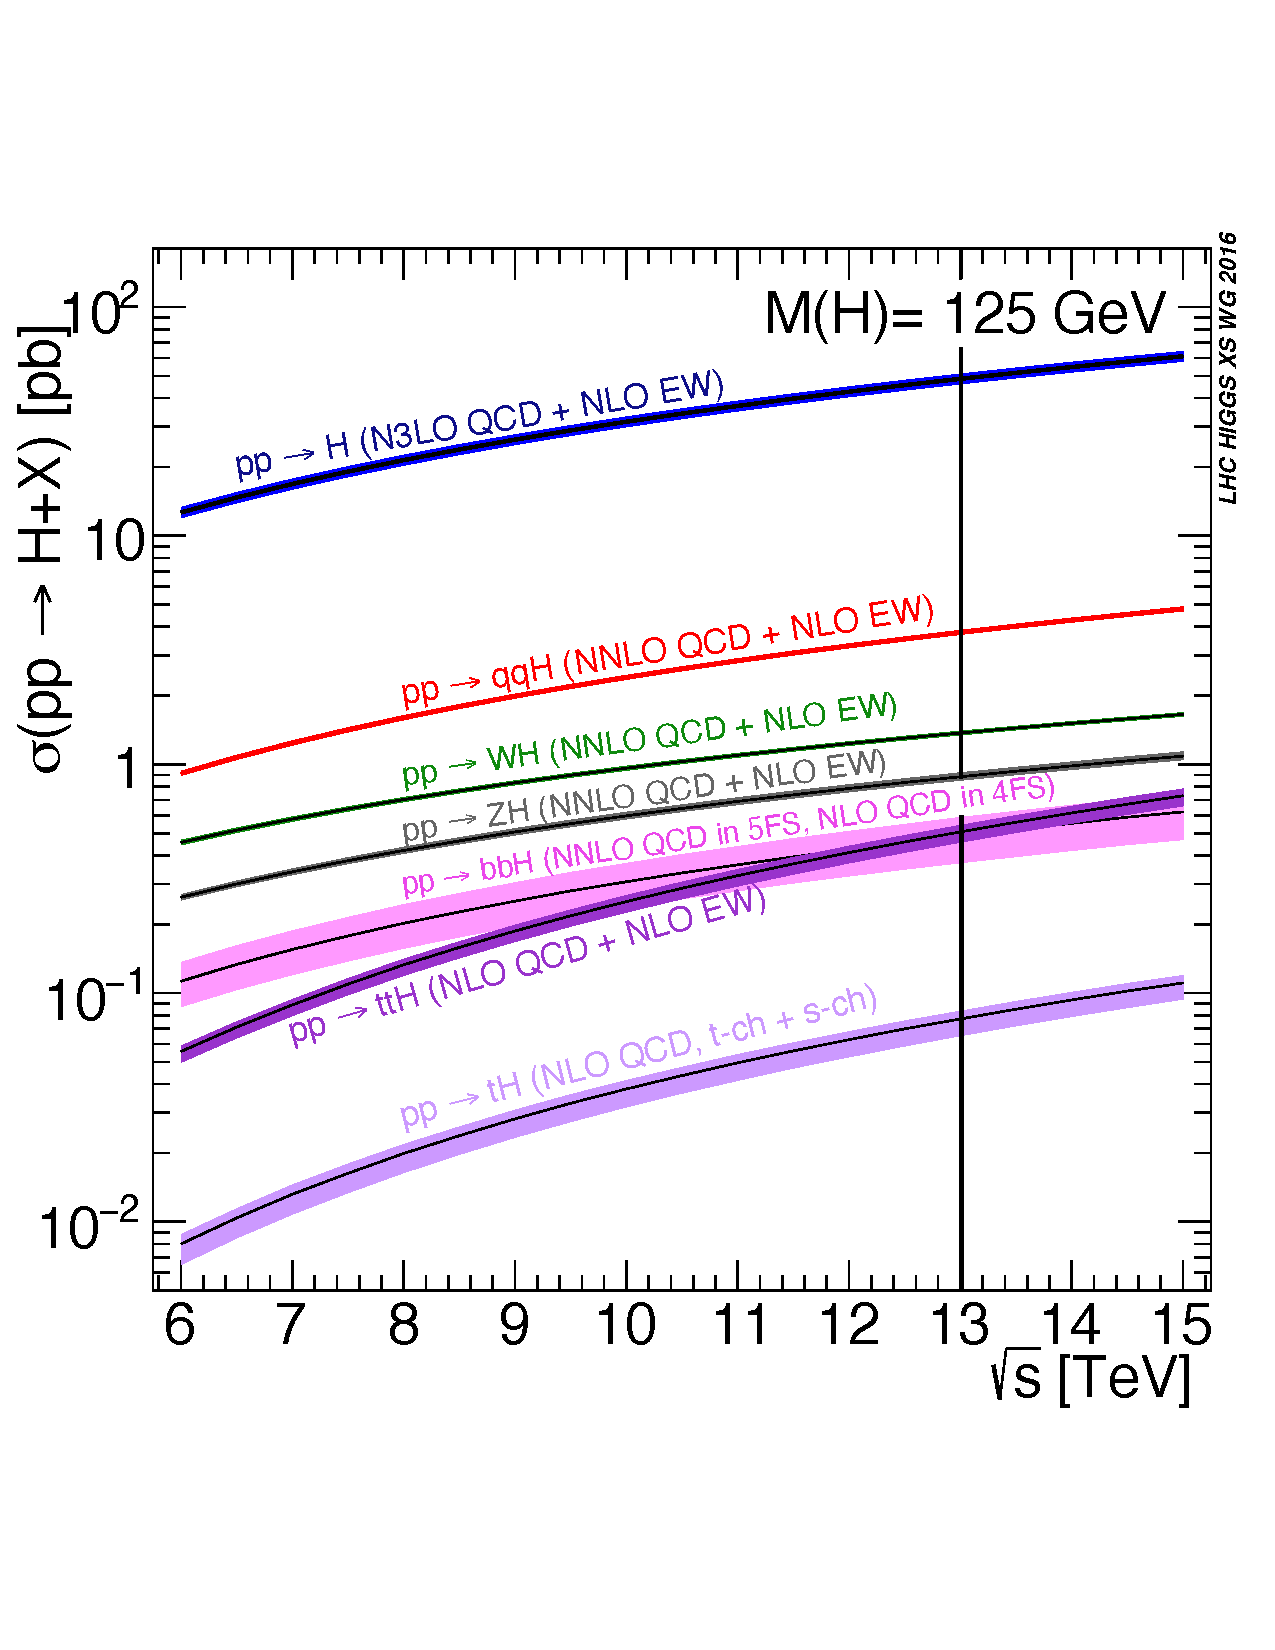
\includegraphics[trim=0 100 0 120, width=0.48\textwidth]{figures/theory/Higgs_Prod_XSec_vertLine_fixed.pdf}
      \label{fig:higgsprodxsec}
    }
    % \hspace{-5em}
    % \captionsetup[subfloat]{captionskip=50pt} % space between subfloat caption and image
    % \subfloat[]{
    %   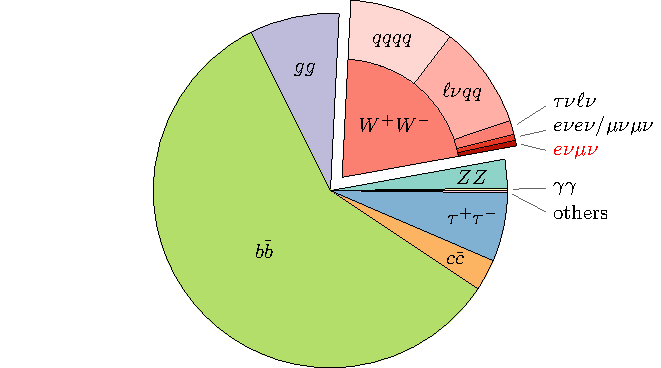
\includegraphics[scale=0.8,valign=t]{figures/theory/h-decay-pie/h-decay-pie.pdf}
    %   \label{fig:higgsbr}
    % }
        \subfloat[]{
            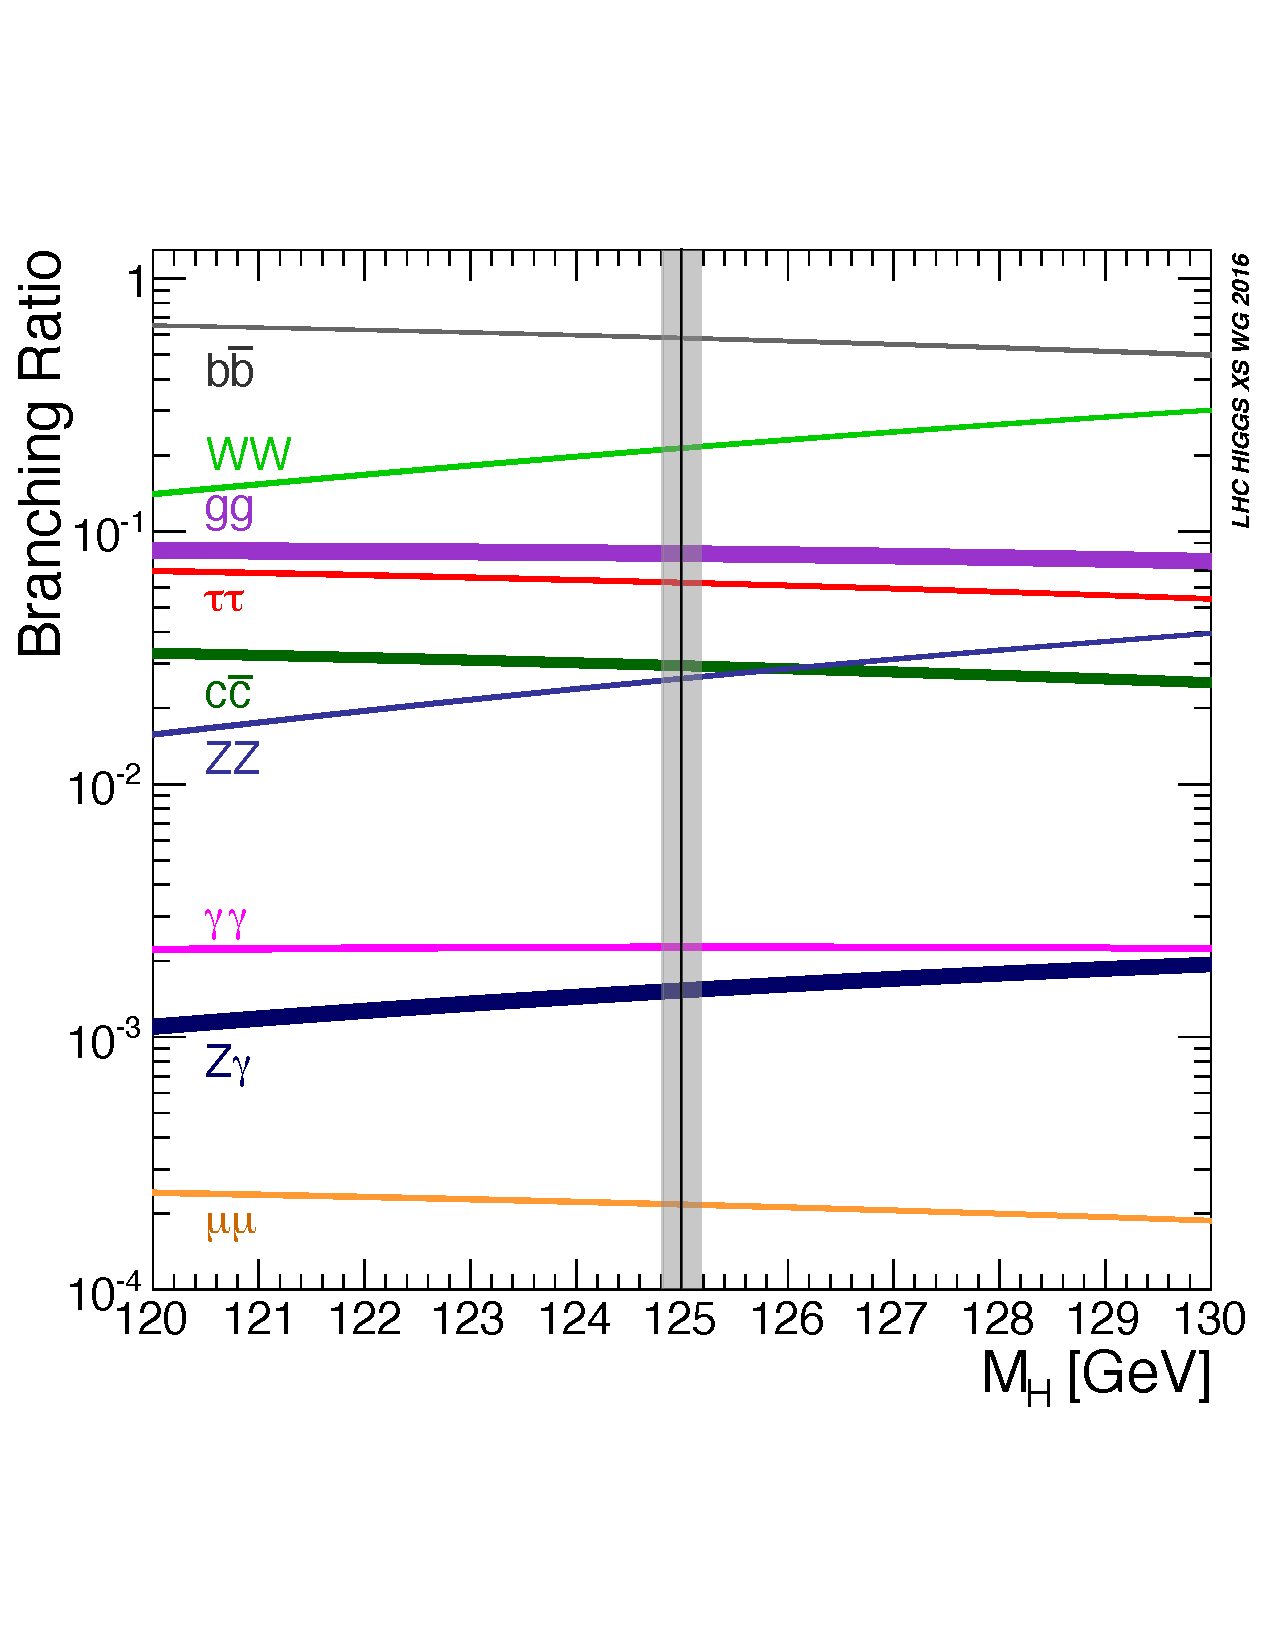
\includegraphics[trim=0 100 0 120, width=0.48\textwidth]{figures/theory/SMHiggsBR_vertLine_fixed.pdf}
            \label{fig:higgsbr}
          }
  \end{center}
  \caption[Higgs boson production cross sections and decay branching fractions.]{(a) Higgs boson production cross sections as a function of the LHC center-of-mass energy and (b) branching fractions of the Higgs boson. The black vertical lines indicate (a) a center-of-mass energy of $\sqrt{s} = 13\,$TeV and (b) the currently measured mass of the Higgs boson including uncertainties by the ATLAS experiment of $m_H = 124.99 \pm 0.19\,\GeV$~\cite{https://doi.org/10.48550/arxiv.2207.00320}. Adapted from Ref.~\cite{deFlorian:2016spz}.}
  % \caption{(a) Higgs boson production cross sections as a function of the LHC center-of-mass energy. The line widths represent the respective theory uncertainties. Taken from Ref.~\cite{deFlorian:2016spz}. (b) branching fractions of the Higgs boson for a mass of 125\,\GeV. Values taken from Ref.~\cite{PDG2020}.}
  %  \label{fig:higgsbr}
\end{figure}

\captionsetup[subfloat]{captionskip=10pt} % space between subfloat caption and image
\begin{figure}
\subfloat[Vector-boson fusion (VBF), $V=W,Z$] {
    \newImageResizeCustom{0.4}{figures/feynman-graphs/Higgs/ProductionModes/VBF.pdf}
}
\subfloat[Gluon fusion (ggF)] {
    \newImageResizeCustom{0.4}{figures/feynman-graphs/Higgs/ProductionModes/ggF.pdf}
} \\
\subfloat[Higgs-strahlung (VH), $V=W,Z$] {
  \newImageResizeCustom{0.4}{figures/feynman-graphs/Higgs/ProductionModes/VH.pdf}
}
\subfloat[$t\bar{t}H$] {
  \newImageResizeCustom{0.4}{figures/feynman-graphs/Higgs/ProductionModes/ttH.pdf}
}
\caption[Feynman diagrams of Higgs boson production.]{Representative Feynman diagrams of the four main production modes of the Higgs boson at the LHC.}
\label{fig:higgsprodfeyn}
\end{figure}
\resetcaptionoffset

\subsection{Experimental sensitivity at the LHC}
\label{subsec:exp-accessibility}
% From PDG
%For a given mH, the sensitivity of a channel depends on the production cross section of the Higgs
% boson, its decay branching fraction, the reconstructed mass resolution, the selection efficiency and
% the level of background in the final state. For a low-mass Higgs boson (110 GeV < mH < 150 GeV)
% for which the SM width would be only a few MeV, five decay channels play an important role
% at the LHC. In the H → γγ and H → ZZ∗ → 4` channels, all final state particles can be
% very precisely measured and the reconstructed mH resolution is excellent (typically 1-2%). While
% the H → W+W− → ` +ν`` 0−ν¯`
% 0 channel has relatively large branching fraction, however, due
% to the presence of neutrinos which are not reconstructed in the final state, the mH resolution,
% obtained through observables sensitive to the Higgs boson mass such as the transverse mass, is poor
% (approximately 20%). The H → b ¯b and the H → τ +τ
% − channels suffer from large backgrounds and
% lead to an intermediate mass resolution of about 10% and 15% respectively.

% PDG
% In order to optimize search sensitivity and also to separate the various Higgs
% boson production modes, ATLAS and CMS split events into several mutually exclusive categories

% For phrasing from PDG
% None of the other production modes have been firmly established by the experiments
% individually. However, the table shows that, for the VBF production mode, the combination had a
% large sensitivity and produced a combined observation of 5.4σ, therefore establishing this process
% with a rate compatible with that expected in the SM.

Physics analyses typically focus on a combination of production and decay mode (referred to as \emph{signal}) to measure the number of Higgs bosons produced. The experimental sensitivity of a particular channel is not only dependent on the respective production cross section and decay branching fraction, but also highly impacted by the signature of the final state. The final state signature determines, for example, how efficient the signal can be reconstructed in the detectors and how well it can be distinguished from other non-Higgs processes considered as \emph{backgrounds}. 
%The different processes are typically first analyzed separately and then combined to obtain the most accurate measurements possible.

%and how well it can be distinguished from other types of events at hadron colliders. 
The $H\rightarrow b\bar{b}$ decay accounts for 58\% of all Higgs boson decays, but the experimental sensitivity to measure this decay mode is limited. The reason is the purely hadronic final state of $H\rightarrow b\bar{b}$ decays. 
This leads to a poor resolution of the mass of the Higgs boson due to the sizable jet energy resolution and also makes it difficult to distinguish the Higgs boson events from QCD multijet events that are extremely abundant at the LHC (see \cref{fig:xsec}).
%from the overwhelming background of QCD events at the LHC. 
The VBF or Higgs-strahlung production modes are therefore typically used where the presence of the additional particles in the final state can be exploited in the event selection.
%It is nonetheless possible to measure this decay by using the VBF or Higgs-strahlung production mode and 
%Using this strategy evidence for the $H\rightarrow b\bar{b}$ decay was recently found in the VH production mode \cite{Aaboud:2017xsd,Sirunyan:2017elk}.\todo{UPDATE}

% The most sensitive channels for the Higgs boson discovery in 2012 were the Higgs boson decays to two photons ($H \to \gamma\gamma$), the $H \to ZZ^* \to llll$, and \HWW\ process.
%Higgs boson initially was discovered in the decay to two photons and the $H \rightarrow ZZ^* \rightarrow llll$ channel \todo{REF}.
The decay into two photons ($H \to \gamma\gamma$) and two $Z$ bosons with a subsequent decay into leptons ($H \to ZZ^* \to llll$) have relatively small branching fractions but exhibit very clean final-state signatures due to the presence of photons and leptons. These decay products can be very precisely measured and allow for a good discrimination of the backgrounds.
In addition, the mass of the Higgs boson can be fully reconstructed in these channels by computing the invariant mass of the reconstructed decay products, providing a well-restricted mass range to measure the signal.
%at a hadron collider, where an overwhelming fraction of events is dominated by QCD effects.
%This is equally important since it allows an excellent selection of signal events and a good control over the background. 
% the largest fraction of events are dominated by QCD effects.
%QCD dominated events
%events at a hadron collider, since the final states are dominated by QCD effects.

The \HWW\ decay also provides a good handle over the backgrounds when selecting leptonically decaying $W$ bosons.
The neutrinos stemming from the $W$ boson decays, however, prevent to fully reconstruct the mass of the Higgs boson, since they cannot be directly detected by the ATLAS experiment.

% Results of the analysis of \HWW\ decays conducted by the ATLAS collaboration and CMS collaboration for data of \RunOne\ can be found in Ref.~\cite{PhysRevD.92.012006} and Ref.~\cite{2013arXiv1312.1129C}, respectively; a corresponding analysis of \RunTwo\ data is given in \cref{sec:ggfanalysis}, focusing on the gluon fusion production-mode.

Events with $H \to \tau\tau $ decays exhibit a similar final state as the \HWW\ process and especially in the case of leptonically decaying $\tau$-leptons allows for an excellent background rejection. 
% htautau paper: https://arxiv.org/abs/2201.08269

The analyses of Higgs boson decays to second generation fermions are challenging, either because of very small branching fractions, as is the case for $H \to \mu\mu$ decays, or because of an overwhelming QCD background, as is the case for $H \to c\bar{c}$ decays.
% 125 considerably more challenging measurements of Higgs boson couplings to second-generation fermions are
% explored via searches for the 𝐻 → 𝜇+𝜇 −
% [32] and, for the first time, 𝐻 → 𝑐𝑐¯ [33] decays.
% From nature:
% The considerably more challenging measurements of Higgs boson couplings to second-generation fermions are explored via searches for the 𝐻 → 𝜇+𝜇−[32] and, for the first time, 𝐻 → 𝑐𝑐¯ [33] decays. Due to the large multijet background, the latter decay mode is currently accessed only via the 𝑊𝐻 and 𝑍𝐻 production. Finally, the inputs to the combination are complemented by the latest direct searches for Higgs boson decays into invisible particles which escape the detector undetected [34, 35].
%Latest cross-section measurements can be found in \todo{REF. Not sure if it's necessary}
%A similar final state as the one in \HWW\ processes, can be exploited when looking at Higgs boson decays into $\tau$-leptons \cite{Aad:2015vsa,Sirunyan:2276465}. 
The Higgs boson decays into $Z\gamma$ ($H \to Z\gamma$) are also very rare and therefore provide limited sensitivity to perform Higgs measurements at the LHC. 
% , where leptonically decaying $Z$ bosons provide the most sensible final state, or $\mu\mu$,  % \cite{Aaboud:2017uhw,Aaboud:2017ojs}.
The final states with gluons ($H \to gg$) make up a considerable fraction of all Higgs decays but are too difficult to differentiate from other events at the LHC due to the overwhelming multijet background and the sizable jet energy resolution. 


\section{Higgs Boson Cross-Section Measurements and Interpretations}
\label{subsec:xsec-measurements}
% From PDG
% For a given mH, the sensitivity of a channel depends on the production cross section of the Higgs boson, its decay branching fraction, the reconstructed mass resolution, the selection efficiency and

% From Peskin/Schroeder
% The experiments that probe the behavior of elementary particles especially in the relativistic regime are scattering experiments. One collides two beams of particles with well dened momenta and observes what comes out The likelihood of any particular final state can be expressed in terms of the cross section, a quantity that is intrinsic to the colliding particles and therefore
% allows comparison of two dierent experiments with dierent b eam sizes and intensities


% From PDG
% In order to optimize search sensitivity and also to separate the various Higgs
% boson production modes, ATLAS and CMS split events into several mutually exclusive categories
The expected cross sections per production mode can be calculated from the SM Lagrangian, once the Higgs boson mass is fixed.
Since the total decay width of the Higgs boson ($\approx 4.1\,\MeV$~\cite{deFlorian:2016spz}) is much smaller than its mass, the narrow-width approximation holds, which allows measuring the Higgs boson cross sections as a product of the production cross section times the branching fractions of the decay modes.
For a given process with final state $f$, the number of observed Higgs boson events is typically expressed in terms of a \emph{signal strength}, defined as 
\begin{equation}
  \label{eq:signal-strength}
  \mu(pp \to H \to f) = \frac{ [ \sigma(pp \to H)  \times \BR(H \to f) ]_\text{meas} } { [ \sigma(pp \to H) \times \BR(H \to f) ]_\text{SM}},
\end{equation}
where the subscript ``meas'' (``SM'') denotes the measured value (prediction of the SM), and $B$ denotes the branching fraction. 

\subsection{Cross-section measurements}
The following briefly outlines the different types of cross-section measurements that are performed in the field of Higgs boson physics. 

% This allows, for example, measuring cross sections in exclusive regions of phase space which improves the resolution with which SM predictions can be probed.
%Differential measurements also allow for easier interpretability of the results, for example in Effective Field Theories (EFT) \todo{REF}.

\subsubsection{Inclusive production cross-section measurements}
Historically, the first measurements of the Higgs boson were based on the total number of Higgs bosons produced per production mode.
These inclusive production mode cross sections are maximally dependent on theoretical assumptions related to the decay properties of the Higgs boson.
They are typically conducted for the search of a new signal (as done for the Higgs boson discovery in 2012) or to experimentally establish different production modes in the SM.
However, inclusive measurements cannot resolve small deviations from the SM predictions that may occur in regions of phase space where only a small fraction of the total produced Higgs bosons are expected.

\subsubsection{Differential fiducial cross-section measurements}
%As more data has been collected at the LHC in recent years, 
In order to probe the SM predictions for different phase space regions exclusively, Higgs boson production processes are measured differentially in various kinematic and topological variables.
Differential measurements use well-defined phase space regions, known as \emph{fiducial regions}, that allow unfolding the detector effects. 
This enables comparisons between experimental data and theory at generator level and thus minimizes the dependency on theoretical assumptions. 
The unfolding is facilitated by relating the expected number of events at detector level to the corresponding number at generator level. It is therefore favored to use simple discriminants for the signal extraction that are well-defined at both detector- and generator level than to use advanced analysis techniques such as neural networks. 
This limits the sensitivity of differential measurements.
% % using advanced analysis techniques for the signal extraction such as neural networks is discouraged. 
% Due to the rather complex unfolding procedure, the use of advanced analysis techniques such as neural networks is discouraged, which limits the sensitivity of differential measurements.
Another drawback is that it is not easily possible to statistically combine differential measurements with different definitions of the fiducial region.  

% - Least theory dependent
% - Not easily possible to combine measurements, as unfolding procedure very tailored to analysis selection. 

\subsubsection{Simplified template cross section measurements}
The \emph{Simplified Template Cross Sections} (STXS) framework provides a way to increase the experimental sensitivity while still allowing for differential measurements of Higgs boson production.
To achieve this, mutually exclusive kinematic regions of Higgs boson production are defined at generator level. They are known as \emph{STXS bins}. 
The extraction of the signal split in these STXS bins is then performed in reconstructed regions, which are typically aligned with the definitions of the STXS bins. This allows using sophisticated analysis techniques like neural networks.
The STXS bins are defined based purely on the production mode and kinematics of the Higgs boson, are agnostic to the different Higgs decay channels, and are agreed upon between experiments.
These design choices allow combining Higgs boson measurements of different decay channels as well as experiments, which enables more precise cross-section measurements.
% The measurements of the production mode cross sections are performed in regions of phase space defined at the level of the fully reconstructed collision events. They are defined as similar as possible to the generator-level bins. This allows using sophisticated analysis techniques like neural networks.

Furthermore, the bins are chosen following two main principles: First, the experimental acceptance is aimed at being constant within each bin, which reduces the dependency on theoretical assumptions. Second, regions that are expected to be sensitive to physics effects beyond the SM are isolated, so that they can be studied separately.
As the amount of available data increases, the STXS binning evolves in stages, each time increasing the number of bins. 
The data from \RunTwo of the LHC allows measuring cross sections partitioned in the Stage 1.2 STXS scheme, which is shown in Appendix~\ref{app:stxs-measurements-aux}.

\subsection{Coupling-strengths measurements and Effective Field Theories}
\label{subsec:coupling-measurements}
Cross-section measurements only probe the production mode of the Higgs boson.
To probe the predicted strengths of the couplings of the Higgs boson to other fundamental particles, the decay processes must also be taken into account.
%A measurement of the Higgs boson's couplings therefore needs to account for both, production and decay processes.
This can be achieved at leading order using the $\kappa$ framework~\cite{LHCHandbookV3}, where the coupling strengths (or simply couplings) are measured by parametrizing the cross sections and branching fractions associated to a particle $j$ in terms of \emph{coupling-strength modifiers}, $\kappa_j^2$.
The cross section times branching fraction in the signal strength of \cref{eq:signal-strength} for a production process $i$ and final state $f$ can then be parametrized as
\begin{equation}
  \label{eq:kappa-parametrization}
  % \left( \sigma \times  \BR \right) (i \to H \to f)  = \kappa_i^2 \times  \kappa_f^2 \times  \sigma_{i}^\mathrm{SM} \times  \frac{\Gamma_f^{\mathrm{SM}}}{\Gamma_H\left(\kappa_i^2, \kappa_f^2\right) }, 
  \left( \sigma \times  \BR \right) (i \to H \to f)  =  \sigma_{i}^\mathrm{SM} \times \BR^\mathrm{SM}(H \to f) \times \frac{\kappa_i^2 \times  \kappa_f^2}{\kappa_H^2}, 
\end{equation}
where $\sigma_{f}^\mathrm{SM}$ and $\BR^\mathrm{SM}(H \to f)$ correspond to the SM expectations. 
The coupling-strength modifiers therefore parametrize deviations from the SM predictions and are unity by definition when the SM is assumed.

The $\kappa$ framework assumes that the data originate from a Higgs boson with a mass of 125\,GeV and the kinematics of both the production and decay are assumed to agree with the SM predictions for the Higgs boson.\footnote{For more details on the assumptions and the parametrization of $\kappa_H$, the reader is referred to \ccite{LHCHandbookV3}.}
The latter assumption, in particular, limits the sensitivity to models beyond the SM that may only affect the SM kinematics. 

An alternative framework to the $\kappa$ framework are interpretations of Higgs boson measurements in Effective Field Theories, for example within the framework of Standard Model Effective Field Theory (SMEFT)\footnote{An overview of SMEFT can, for example, be found in \ccite{Brivio_2019}.}.
In SMEFT, the effects of physics beyond the SM at large energy scales $\Lambda$ -- large compared to the Higgs vacuum expectation value ($\Lambda \gg v$) -- are parametrized at low energies, $E \ll \Lambda$, in terms of effective couplings. 
This allows for a theory-independent approach to search for deviations of the SM, and relies on fewer assumptions than the $\kappa$ framework. 

% For the VBF, \HWW process, the modifiers become
% \begin{align}
%   \label{eq:kappa-parametrization-VBF}
%   \kappa_i^2 &= \kappa_\mathrm{VBF}^2 = 0.733 \kappa^2_W + 0.267 \kappa^2_Z, \\
%   \kappa_f^2 &= \kappa_W^2, 
%   % \sigma_{\mathrm{VBF}} \cdot \BR (H \to WW)  = \kappa_\mathrm{VBF}^2 \cdot \kappa_W^2 \cdot \sigma_{\mathrm{VBF}}^\mathrm{SM} \frac{\Gamma_{WW}^\mathrm{SM}}{\Gamma_H\left(\kappa_\mathrm{VBF}^2, \kappa_{W}^2\right) },
% \end{align}
% where the parametrization of $\kappa_\mathrm{VBF}^2$ corresponds to the one used in \ccite{NaturePaper}.
% The latter shows, that a set of assumptions must be made in the $\kappa$-framework, since the couplings cannot be directly accessed. 
% Typically, different parametrizations and scenarios are tested in the couplings measurements. 
% More details left to \ccite{LHCHandbookV3}.
% Because the couplings cannot be directly measured, a set of assumptions must be made in the framework.
% For example, the framework assumes that the data originate from a Higgs boson with a mass of 125\,GeV and its interactions are exactly as predicted by the SM.
% More details on the framework are provided in \ccite{LHCHandbookV3}.
% To this end, the couplings of the Higgs boson to individual particles can be measured by scaling the cross sections and branching fractions for the individual Higgs boson processes in terms of coupling-strength modifiers, $\kappa$. 
%To this end, the $\kappa$ framework~\cite{LHCHandbookV3} parametrizes the signal strengths 
% The couplings of the Higgs boson to individual particles can be measured by parametrizing the cross sections and branching fractions for the individual Higgs boson processes in terms of coupling-strength modifiers, $\kappa$, following the $\kappa$-framework~\cite{LHCHandbookV3}. 
% \subsection{Properties of HWW Decays}
% % THIS MIGHT actually fit in the analysis section
% % as it directly related to what analysis selections we perform
% % THINK ABOUT IT!
% - VBF Higgs -> ww cross section must be exactly the SM value, otherwise VBS xsec converges!
% -> Maybe add this to HWW analysis

\section{Current Experimental Status}
\label{subsec:higgs-exp-status}
% All experimentally accessible decay modes of the Higgs have been observed, which includes $H \to \gamma\gamma$, $H \to ZZ$, $H \to WW$, $H \to \tau\tau$, and $H \to b\bar{b}$. 
After the discovery of a particle consistent with the Higgs boson predicted by the SM in 2012~\cite{HIGG-2012-27,CMS-HIG-12-028}, an era of Higgs boson precision physics has started.
The data from \RunOne\ and \RunTwo\ of the LHC allowed for high-precision measurements of several properties of the Higgs boson such as its mass, width, spin, or parity, as well as Higgs boson production and decay processes. 
At the time of writing, all experimental measurements are consistent with the predictions of the SM.
This section briefly summarizes the current experimental status, mostly focusing on results of the ATLAS collaboration.
% This allows placing the measurements presented in this thesis in a broader context. 
A more comprehensive overview can be found in \ccite{PDG2020}. 
%allowing to place the work presented in this thesis into a broader context. 

\subsection{Higgs boson properties}
% The latest combined measurement of the ATLAS and CMS experiment~\cite{HIGG-2014-14} measures a Higgs boson mass of 
% \begin{equation}
%   m_H = 125.09 \pm 0.21\text{(stat.)} \pm 0.11\text{(syst.)}\,\GeV.
% \end{equation}
The most recent measurements of the Higgs boson mass performed by the ATLAS and CMS collaboration measure a mass of $m_H = 124.99 \pm 0.19\,\GeV$~\cite{https://doi.org/10.48550/arxiv.2207.00320} and $m_H = 125.38 \pm 0.14\,\GeV$~\cite{CMS-HIG-19-004}, respectively.
Measurements of the spin and parity of the Higgs boson confirm the SM predictions of a spin-parity $J^{P} = 0^{+}$ and exclude alternative hypothesis beyond 99.9\% confidence level (CL)~\cite{HIGG-2013-17-witherratum,CMS-HIG-14-018}.
The CP-even hypothesis for the SM Higgs boson has also been probed for several interactions and all measurements are in agreement with the CP-even prediction (see e.g. \ccite{ATLAS-CONF-2022-032,Aad_2020CP,CMS-HIG-17-011}).
The total width of the Higgs boson in the SM is small ($\Gamma_H^{\text{SM}} = 4.1\,$ MeV~\cite{deFlorian:2016spz}) and therefore difficult to measure directly at hadron colliders. Indirect measurements using off-shell production of Higgs bosons result in a measured width of $\Gamma_H = 3.2 ^{+2.4}_{-1.7}\,$ MeV~\cite{https://doi.org/10.48550/arxiv.2202.06923}.

\subsection{Higgs boson production and decay processes}
All major Higgs boson production modes (ggF, VBF, $VH$, $ttH$) and Higgs boson decays to bosons ($H \to WW$, $H \to ZZ$, $H \to \gamma\gamma$) as well as third-generation fermions ($H \to \tau^+\tau^-$, $H \to b\bar{b}$) have been observed at the LHC with significances larger than $5\,\sigma$ above the background expectation~\cite{NaturePaper}.
While precision measurements are now being performed for these channels, rarer Higgs boson processes have not been unambiguously confirmed with the data available ($H \to Z\gamma$; and decays to second-generation fermions $H \to \mu^+\mu^-$, $H \to c\bar{c}$) or remain experimentally out of reach at the LHC ($H \to s\bar{s}$; decays to first-generation fermions $H \to e^+e^-$, $H \to u\bar{u}$, $H \to d\bar{d}$; and decays to gluons $H \to gg$).

A combination of several individual Higgs boson measurements using many of the above-mentioned production and decay modes of the Higgs boson was recently performed by the ATLAS collaboration~\cite{NaturePaper}. 
The combination includes the \HWW\ analysis that is presented in detail in \cref{chap:hww} of this thesis, which is why a summary of the combined measurements is left to \cref{chap:comb}. 
They provide the most precise measurements to date of the production and decay of the Higgs boson and the couplings of the Higgs boson to other fundamental particles. 

Rare decay modes of the Higgs boson begin to emerge from the data of \RunTwo\ of the LHC. 
The search for Higgs decays to a pair of muons of the ATLAS experiment found an excess of $H \to \mu\mu$ events over the background expectation of 2.0 standard deviations, where 1.7 were expected~\cite{HIGG-2019-14}.
The CMS collaboration found evidence for the $H \to \mu\mu$ decay~\cite{CMSHmumuevidence}.
An analysis of $H \to cc$ events yields an observed (expected) upper limit of 26 (31) times the SM prediction~\cite{ATLAS-CONF-2021-021}, and a search for $H \to Z\gamma$ decays results in an observed (expected) upper limit of 3.6 (2.6) times the SM prediction~\cite{HIGG-2018-42}.
An upper limit on the branching fraction of Higgs decays to particles that are invisible to the detector was set to 0.145, where 0.103 was expected~\cite{ATLASInvisible1}.
The cross section of double Higgs boson production is extremely low. The most stringent upper limits by the ATLAS collaboration were set to 4.1 times the SM prediction at 95\% CL using $HH \to b\bar{b}\gamma\gamma$ decays~\cite{ATLAS-CONF-2021-016}.
%Other search to invisible: \cite{Aad_2022}
% From nature
% Even with the current precision of measurements there is room for possible interpretations of the data in terms of new phenomena beyond the SM. 
% From nature
% Finally, the inputs to the combination are complemented by the latest direct searches for Higgs boson
% 129 decays into invisible particles which escape the detector undetected [34, 35].

\subsection{Differential measurements and interpretations in Effective Field Theories}
The \RunTwo\ data of the LHC also allowed measuring differential fiducial cross sections of Higgs boson production. Analyses targeting the $H \to ZZ$ decay~\cite{ATLAS:2020wny} and $H \to \gamma\gamma$ decay~\cite{hgammagammaDiff} measured cross sections for a variety of observables sensitive to the production and decay processes of the Higgs boson, and set constraints on beyond the SM effects.
%(THEORETICALLY there is a combination of the above here: ATLAS-CONF-2022-002)
% Measurements of Higgs boson production cross sections also serve as basis for further interpretation, for example within the framework of Standard Model Effective Field Theory (SMEFT)\footnote{An overview of SMEFT can, for example, be found in \ccite{}.}. In SMEFT, the effects of physics beyond the SM at large energy scales $\Lambda$ -- large compared to the Higgs vacuum expectation value ($\Lambda \gg v$) -- are parametrized at low energies, $E \ll \Lambda$, in terms of effective couplings. 
% This allows for a theory-independent approach to search for deviations of the SM. 

A combination of different Higgs boson cross-section measurements was interpreted in the SMEFT framework by the ATLAS collaboration~\cite{ATLAS-CONF-2020-053}. This also allowed setting constraints on new physics models.
As well, the ATLAS collaboration combined the analysis of \HWW\ decays with differential cross-section measurements of $WW^*$ production in order to interpret the measured cross sections in terms of effective couplings~\cite{ATL-PHYS-PUB-2021-010}.
Both of these results pave the way for future interpretations of Higgs boson measurements in Effective Field Theories. %which become especially important in the absence of any direct discovery of new particles. 

% % The latest combined Higgs measurements performed by the ATLAS collaboration of the kinematic properties of Higgs boson production, as well as the Higgs coupling to other particles, are nicely summarized in \ccite{NaturePaper}.

% In addition to the results presented in \ccite{NaturePaper}, Higgs analyses can be interpreted in the framework of Effective Field Theories. 
% Effective field theories parametrise...
% They allow for a general parametrisation of deviations of the SM. 
% %Differential measurements also allow for easier interpretability of the results, for example in Effective Field Theories (EFT).


%%%%%%%%%%%%%%%%%%%
% Maybe not the following!
%%%%%%%%%%%%%%%%%%%

% \subsection{Cross-section measurements of \HWW decays}
% \label{subsec:prev-hwww-cross-section-meas}

% The \HWW process was first observed using data from \RunOne of the LHC~\cite{HIGG-2013-13}, and an analysis of a partial \RunTwo dataset corresponding to 36.1\,\ifb\ reported the most recent ggF and VBF \HWW measurements~\cite{HIGG-2013-13}.
% In the analysis presented here, several improvements compared to the previous \RunTwo results are implemented. Most noteworthy, the discrimination of the VBF signal is performed using a deep neural network (DNN) instead of a boosted decision tree, ggF signal events with two or more jets in the final state are included in the measurement, and measurements of cross sections in the kinematic regions defined by the STXS framework (\emph{STXS measurement}) are reported for the first time for this process.
% The analysis is published in \ccite{HWWPaper} and yields some of the most precise Higgs cross-section meausurements to date.




